%%
%% Copyright 2022 OXFORD UNIVERSITY PRESS
%%
%% This file is part of the 'oup-authoring-template Bundle'.
%% ---------------------------------------------
%%
%% It may be distributed under the conditions of the LaTeX Project Public
%% License, either version 1.2 of this license or (at your option) any
%% later version.  The latest version of this license is in
%%    http://www.latex-project.org/lppl.txt
%% and version 1.2 or later is part of all distributions of LaTeX
%% version 1999/12/01 or later.
%%
%% The list of all files belonging to the 'oup-authoring-template Bundle' is
%% given in the file `manifest.txt'.
%%
%% Template article for OXFORD UNIVERSITY PRESS’s document class `oup-authoring-template'
%% with bibliographic references
%%

%%%CONTEMPORARY%%%
\documentclass[unnumsec,webpdf,contemporary,large]{oup-authoring-template}%
%\documentclass[unnumsec,webpdf,contemporary,large,namedate]{oup-authoring-template}% uncomment this line for author year citations and comment the above
%\documentclass[unnumsec,webpdf,contemporary,medium]{oup-authoring-template}
%\documentclass[unnumsec,webpdf,contemporary,small]{oup-authoring-template}

%%%MODERN%%%
%\documentclass[unnumsec,webpdf,modern,large]{oup-authoring-template}
%\documentclass[unnumsec,webpdf,modern,large,namedate]{oup-authoring-template}% uncomment this line for author year citations and comment the above
%\documentclass[unnumsec,webpdf,modern,medium]{oup-authoring-template}
%\documentclass[unnumsec,webpdf,modern,small]{oup-authoring-template}

%%%TRADITIONAL%%%
%\documentclass[unnumsec,webpdf,traditional,large]{oup-authoring-template}
%\documentclass[unnumsec,webpdf,traditional,large,namedate]{oup-authoring-template}% uncomment this line for author year citations and comment the above
%\documentclass[unnumsec,namedate,webpdf,traditional,medium]{oup-authoring-template}
%\documentclass[namedate,webpdf,traditional,small]{oup-authoring-template}

%\onecolumn % for one column layouts

%\usepackage{showframe}

\graphicspath{{doc/}}

% line numbers
%\usepackage[mathlines, switch]{lineno}
%\usepackage[right]{lineno}

\theoremstyle{thmstyleone}%
\newtheorem{theorem}{Theorem}%  meant for continuous numbers
%%\newtheorem{theorem}{Theorem}[section]% meant for sectionwise numbers
%% optional argument [theorem] produces theorem numbering sequence instead of independent numbers for Proposition
\newtheorem{proposition}[theorem]{Proposition}%
%%\newtheorem{proposition}{Proposition}% to get separate numbers for theorem and proposition etc.
\theoremstyle{thmstyletwo}%
\newtheorem{example}{Example}%
\newtheorem{remark}{Remark}%
\theoremstyle{thmstylethree}%
\newtheorem{definition}{Definition}

\begin{document}

\journaltitle{Journal Title Here}
\DOI{DOI HERE}
\copyrightyear{2024}
\pubyear{2019}
\access{Advance Access Publication Date: Day Month Year}
\appnotes{Paper}

\firstpage{1}

%\subtitle{Subject Section}

\title[SNF-CNN, comprehensive DDI prediction]{SNF-CNN: Predicting Comprehensive Drug-Drug Interaction via Similarity Network Fusion and Convolutional Neural Networks}
% [1,4,$\ast$]
\author[1,3]{M.Amin Khodamoradi\ORCID{0000-0002-2700-5384}}
\author[2]{ Bahareh Levian}
\author[2]{Changiz Eslahchi}
\author[3]{Maria Marques}
\author[1,3]{Ricardo Jardim-Gonçalves}
% \author[4]{Fifth Author\ORCID{0000-0000-0000-0000}}

\authormark{A. Khodamoradi et al.}

\address[1]{\orgdiv{Universidade NOVA de Lisboa}, \orgname{NOVA School of Science and Technology (FCT NOVA)}, \orgaddress{\state{Caparica}, \country{Portugal}}}
\address[2]{\orgdiv{Department of Computer Sciences}, \orgname{Shahid Beheshti University}, \orgaddress{\state{Tehran}, \country{Iran}}}

\address[3]{
\orgdiv{Center of Technology and Systems (UNINOVA-CTS) and Associated Lab of Intelligent Systems (LASI)}, \orgname{Organization}, \orgaddress{\state{Caparica}, \country{Portugal}}}

% \corresp[$\ast$]{Corresponding author. \href{email:Khodamoradi1992@gmail.com}{Khodamoradi1992@gmail.com}}

\received{Date}{0}{Year}
\revised{Date}{0}{Year}
\accepted{Date}{0}{Year}

%\editor{Associate Editor: Name}

%\abstract{
%\textbf{Motivation:} .\\
%\textbf{Results:} .\\
%\textbf{Availability:} .\\
%\textbf{Contact:} \href{name@email.com}{name@email.com}\\
%\textbf{Supplementary information:} Supplementary data are available at \textit{Journal Name}
%online.}

\abstract{
\textbf{Motivation:} This research addresses the critical need to identify drug-drug interactions (DDIs) before market entry. Existing preclinical detection methods are resource-intensive, prompting the use of computational models based on premarket drug properties. However, current models often oversimplify interactions, neglecting nuanced alterations in pharmacological effects. DDIs, rooted in the structural features of the DDI graph, are non-random, and understanding these relationships is vital for making comprehensive predictions and uncovering structural patterns in the DDI graph. This study introduces the Similarity Network Fusion and Convolutional Neural Networks (SNF-CNN) model, treating comprehensive DDIs as a signed network. \\
\textbf{Results:} SNF-CNN excels in predicting degressive (AUC = 0.975, AUPR = 0.967), enhancive (AUC = 0.969, AUPR = 0.822) and Unknown DDIs (AUC = 0.971, AUPR = 0.948). A comparative analysis against state-of-the-art methods highlights the superiority of SNF-CNN, not only in predicting DDIs but also in accurately forecasting non-DDIs. The graphical abstract of SNF-CNN is provided (Figure~\ref{graphabs}).\\
\textbf{Availability and implementation:} The SNF-CNN and data are available as open-source from GitHub at: \href{https://github.com/aminkhod/SNF-CNN}{https://github.com/aminkhod/SNF-CNN}. 
\\
For inquiries or collaboration, please contact \href{mailto: A.khodamoradi@uninova.pt}{A.khodamoradi@uninova.pt}.
% \textbf{Motivation}: Identifying drug-drug interactions (DDIs) before market entry is critical. While preclinical detection is resource-intensive, computational methods predict DDIs based on premarket drug properties. Existing models often focus on binary interactions, overlooking nuanced alterations in pharmacological effects. DDIs, rooted in the structural features of the DDI graph, are not random. Uncovering these relationships is crucial for understanding DDI mechanisms, guiding comprehensive predictions, and revealing structural patterns in the DDI graph for prescribing multiple drugs.\\
% Drug-drug interactions (DDIs) often lead to unexpected and adverse reactions, underscoring the critical need for their identification before market entry. However, preclinical detection of DDIs remains resource-intensive. Computational methods have demonstrated the ability to predict potential DDIs on a large scale using premarket drug properties. While many models focus on determining whether drugs interact, they frequently overlook the enhancive (positive) and degressive (negative) alterations of pharmacological effects. Furthermore, these complex DDIs are not random and may stem from the structural features of the DDI graph. Uncovering such relationships is essential for understanding the mechanisms behind DDI occurrences. Predicting comprehensive DDIs and elucidating structural patterns in the DDI graph provide crucial guidance for prescribing multiple drugs.\\
% \textbf{Results}: In this study, we treat a set of comprehensive DDIs as a signed network and introduce the Similarity Network Fusion and Convolutional Neural Networks (SNF-CNN) model for predicting the enhancive or depressive effects of drug pairs. SNF-CNN demonstrates strong performance in depressive DDI prediction (AUC = 0.975, AUPR = 0.967), enhancive DDI prediction (AUC = 0.969, AUPR = 0.822), and Unknown DDI prediction (AUC = 0.971, AUPR = 0.948). Comparative analysis against three state-of-the-art methods on our dataset highlights the superiority of SNF-CNN. This innovative approach excels not only in predicting comprehensive DDIs but also in accurately forecasting non-DDIs.\\
% \textbf{Availability and Implementation}: The code and data are available on the GitHub page of \href{https://github.com/aminkhod/DDI-Project}{SNF-CNN code and data} (\url{https://github.com/aminkhod/DDI-Project})\\
% \textbf{Contact}: \href{mailto: A.khodamoradi@uninova.pt}{A.khodamoradi@uninova.pt}\\
% \textbf{Supplementary Information} Links to additional figures/data available on a website or reference to online-only supplementary data available at the journal’s website.\\
\begin{figure}[H]
\scriptsize
% \centering
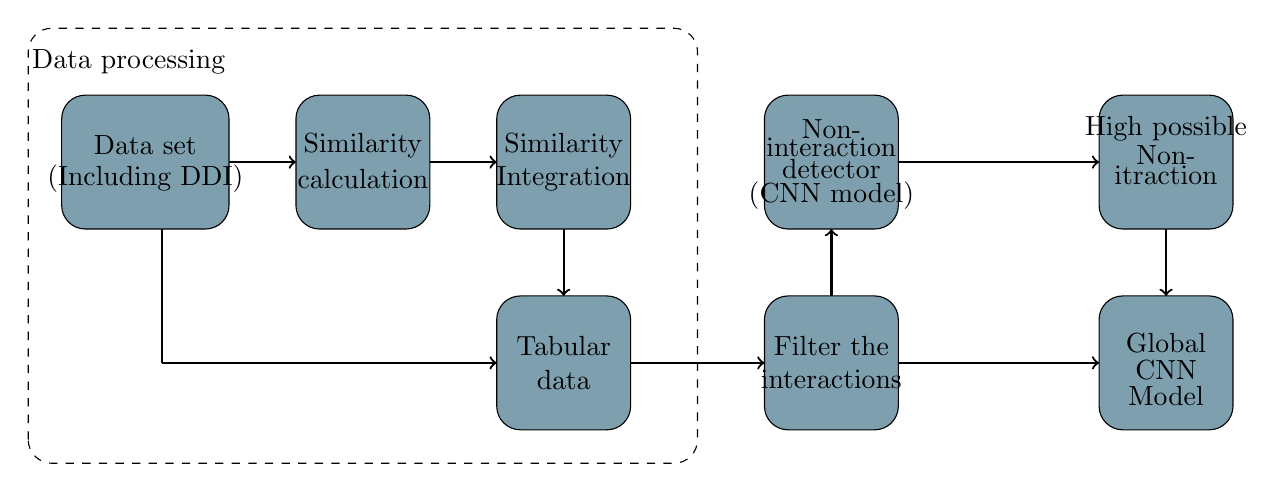
\begin{tikzpicture}[scale=.85, inner sep=0]
% [scale=0.9]
% Define the nodes
% \node[rotate=90] (ddi) at (-0.5,2) {Data set};
\draw[rounded corners=3mm, dashed] (-1, -2.5) rectangle (9, 4);
\node[inner sep=0pt] (ddi) at (0.5,3.5) {Data processing};
\draw[rounded corners=3mm, fill=cyan!30!gray] (-0.5, 1) rectangle (2, 3);
% \draw[rounded corners=3mm, fill=cyan!40!gray] (0, 0) rectangle (2, 1);
% \draw[rounded corners=3mm, fill=cyan!40!gray] (0, 1.5) rectangle (2, 2.5);
% \draw[rounded corners=3mm, fill=cyan!40!gray] (0, 3) rectangle (2, 4);
\node[inner sep=0pt] (ddi) at (0.75,2.25) {Data set};
\node[inner sep=0pt] (ddi) at (0.75,1.75) {(Including DDI)};
% \node[inner sep=0pt] (fs) at (1,2) {$F_{Str}$};
% \node[inner sep=0pt] (fo) at (1,3.5) {$F_{se}$};
\draw[rounded corners=3mm, fill=cyan!30!gray] (3, 1) rectangle (5, 3);
\node[inner sep=0pt] (conv2d_1) at (4,2.25) {\text{Similarity}};
\node[inner sep=0pt] (conv2d_1) at (4,1.75) {\text{calculation}};
% \draw[rounded corners=3mm, fill=cyan!30!gray] (6, 0) rectangle (8, 1.5);
% \node[inner sep=0pt] (conv2d_1) at (7,0.75) {$S_{Str}$};
% \draw[rounded corners=3mm, fill=cyan!30!gray] (6, 2.5) rectangle (8, 4);
% \node[inner sep=0pt] (conv2d_1) at (7,3.25) {$S_{se}$};
\draw[rounded corners=3mm, fill=cyan!30!gray] (6, 1) rectangle (8, 3);
\node[inner sep=0pt] (conv2d_1) at (7,2.25) {\text{Similarity}};
\node[inner sep=0pt] (conv2d_1) at (7,1.75) {\text{Integration}};
\draw[rounded corners=3mm, fill=cyan!30!gray] (6, -2) rectangle (8, 0);
\node[inner sep=0pt] (conv2d_1) at (7,-0.75) {\text{Tabular}};
\node[inner sep=0pt] (conv2d_1) at (7,-1.25) {\text{data}};
\draw[rounded corners=3mm, fill=cyan!30!gray] (10, -2) rectangle (12, 0);
\node[inner sep=0pt] (conv2d_1) at (11,-0.75) {\text{Filter the }};
\node[inner sep=0pt] (conv2d_1) at (11,-1.25) {\text{interactions}};
\draw[rounded corners=3mm, fill=cyan!30!gray] (10, 1) rectangle (12, 3);
\node[inner sep=0pt] (conv2d_1) at (11,2.5) {\text{Non-}};
\node[inner sep=0pt] (conv2d_1) at (11,2.22) {\text{interaction}};
\node[inner sep=0pt] (conv2d_1) at (11,1.9) {\text{detector}};
\node[inner sep=0pt] (conv2d_1) at (11,1.5) {\text{(CNN model)}};
\draw[rounded corners=3mm, fill=cyan!30!gray] (15, -2) rectangle (17, 0);
\node[inner sep=0pt] (conv2d_1) at (16,-0.7) {\text{Global}};
\node[inner sep=0pt] (conv2d_1) at (16,-1.1) {\text{CNN}};
\node[inner sep=0pt] (conv2d_1) at (16,-1.5) {\text{Model}};
\draw[rounded corners=3mm, fill=cyan!30!gray] (15, 1) rectangle (17, 3);
\node[inner sep=0pt] (conv2d_1) at (16,2.5) {\text{High possible}};
\node[inner sep=0pt] (conv2d_1) at (16,2.1) {\text{Non-}};
\node[inner sep=0pt] (conv2d_1) at (16,1.8) {\text{itraction}};
% \node[inner sep=0pt] (x2) at (9.5,0.5)
%     {\text{{$\boldsymbol{x}(k+2)$}}};
\draw[-, thick] (1, 1) -- (1, -1);  
\draw[->, thick] (1, -1) -- (6, -1); 
\draw[->, thick] (2, 2) -- (3, 2);
\draw[->, thick] (5, 2) -- (6, 2);
% \draw[->, thick] (2, 3.5) -- (3, 2); 
% \draw[->, thick] (5, 2) -- (6, 3); 
% \draw[->, thick] (5, 2) -- (6, 1); 
% \draw[->, thick] (8, 1) -- (9, 2); 
% \draw[->, thick] (8, 3) -- (9, 2);
\draw[->, thick] (7, 1) -- (7, 0);
\draw[->, thick] (8, -1) -- (10, -1);
\draw[->, thick] (12, -1) -- (15, -1);
\draw[->, thick] (12, 2) -- (15, 2);
\draw[->, thick] (11, 0) -- (11, 1);
\draw[->, thick] (16, 1) -- (16, 0);
\end{tikzpicture}
\caption{Graphical abstract}
\label{graphabs}
\end{figure}}
\keywords{Drug-Drug Interaction, Drug Similarity, Drug Similarity Integration, Feature Selection, Recommender System}
% \boxedtext{
% \begin{itemize}
% \item Key boxed text here.
% \item Key boxed text here.
% \item Key boxed text here.
% \end{itemize}}
\Abbreviations{DDI:Drug-drug interactions; CV:cross-validation; SNF:Similarity Network Fusion}

\maketitle
\section{Introduction}
% When two or more drugs are taken together, drugs’ effects or behaviors might be unexpectedly influenced by each other~\cite{Wienkers2005}. This kind of influence is termed Drug-Drug interaction (DDI), which may reduce drug efficacy, increase unexpected toxicity, or induce other adverse drug reactions between the co-prescribed drugs. As the number of approved drugs increases, the number of drug-unidentified DDIs is rapidly increasing, such that among approved small molecular drugs in Drug Bank\footnote{\url{ https://go.drugbank.com}}, on average, $15$ out of every $100$ drug pairs have known DDIs~\cite{Law2014}. The DDI may put patients who are treated with multiple drugs in an unsafe situation~\cite{Leape1995, PMID:28232141, Mulroy2017}. Understanding DDI is the first step in drug combinations, which has become one of the most promising solutions for treating multifactorial complex diseases~\cite{PMID:22219721}. Therefore, there is an urgent need for screening and analysis of DDIs before clinical co-medications are administered. However, traditional DDI identification approaches (e.g., testing Cytochrome P450~\cite{Veith2009} or transporter-associated interactions~\cite{Huang2007}) face challenges, such as high costs, long duration, animal welfare considerations~\cite{Zhang2015}, the very limited number of participants in trials, and a great number of drug combinations under screening in clinical trials. As a result, only a few DDIs have been identified during drug development production (usually in the clinical trial phase). Some of them have been reported after drugs were approved, and many have been found in post-marketing surveillance~\cite{Karim2019}. 
When multiple drugs are taken together, their effects or behaviors may be unexpectedly influenced by each other~\cite{Wienkers2005}. This phenomenon is known as Drug-Drug Interaction (DDI), which can lead to reduced drug efficacy, increased toxicity, or other adverse reactions between the co-prescribed drugs. With the rising number of approved drugs, the incidence of unidentified DDIs is snowballing. For instance, among approved small molecular drugs listed in the DrugBank, approximately 15 out of every 100 drug pairs have known DDIs~\cite{Law2014}. Such interactions pose risks to patients receiving multiple medications~\cite{Leape1995, PMID:28232141, Mulroy2017}. Understanding DDI is crucial as it is the first step in exploring drug combinations, which are increasingly seen as promising solutions for treating complex diseases~\cite{PMID:22219721}. Therefore, there is an urgent need for screening and analyzing DDIs before administering clinical co-medications. However, traditional DDI identification approaches, such as testing Cytochrome P450~\cite{Veith2009} or transporter-associated interactions~\cite{Huang2007}, face challenges including high costs, time consumption, animal welfare concerns~\cite{Zhang2015}, limited trial participants, and a multitude of drug combinations undergoing screening in clinical trials. Consequently, only a few DDIs are identified during drug development, often in the clinical trial phase. Some are reported post-approval, while many are discovered during post-marketing surveillance~\cite{Karim2019}.
% DDIs can be significantly affected by a patient’s medical history [a] and genetics [b]. To facilitate the link between these aspects, the Smart4Health project\footnote{\url{http://www.smart4health.eu}} developed two platforms: one personal, containing health information from the citizen (Citizen Health Data Platform – CHDP) such as medical conditions, allergies, and intolerances, medication use, as well as genetic data, and one deidentified, containing data donated for research by the citizen (Research Platform – RP). While CHDP adopts HL7 FHIR\footnote{\url{ https://hl7.org/fhir}} to structure collected data, RP follows OMOP CDM\footnote{\url{https://www.ohdsi.org/data-standardization}} to convey data coming from CHDP and make it reusable by third-party research infrastructures (e.g., ELIXIR\footnote{\url{https://elixir-europe.org}}). The concept of use entails the possibility of a citizen collecting and aggregating aggregate data generated from interactions with medical institutions (e.g., medication prescriptions, laboratory results, discharge letters, etc.) into one single, interoperable HER. This data may also include genetic data if available. At citizens' discretion, this data can be donated to the RP. In the specific case of data related to medication intake and genetic data, these are linked to drug exposure and outcome data within the OMOP CDM. This mechanism has the potential to facilitate data collection and contribute to ensuring the quality of the collected data. In addition, having the citizen at the center of this process may accelerate and expand the identification of DDIs, enabling a more comprehensive understanding of their mechanisms.
DDI can be significantly influenced by a patient’s medical history and genetics. To bridge these aspects, the Smart4Health project\footnote{\url{http://www.smart4health.eu}} developed two platforms: one personal, containing health information from the citizen (Citizen Health Data Platform – CHDP), including medical conditions, allergies, intolerances, medication use, and genetic data, and one de-identified, containing data donated by the citizen for research (Research Platform – RP). CHDP utilizes the Health Level Seven (HL7®) Fast Healthcare Interoperability Resources (FHIR®) standard\footnote{\url{ https://hl7.org/fhir}} to structure collected data, while RP adopts Observational Medical Outcomes Partnership (OMOP) Common Data Model (CDM) to convey data from CHDP and make it reusable by third-party research infrastructures (e.g., ELIXIR\footnote{\url{https://elixir-europe.org}}). The concept involves citizens collecting and aggregating data generated from interactions with medical institutions (e.g., medication prescriptions, laboratory results, discharge letters) into a single, interoperable EHR. This data may also encompass genetic data if available. This data can be donated to the RP at the citizens' discretion. Specifically regarding medication intake and genetic data, these are linked to drug exposure and outcome data within the OMOP CDM\footnote{\url{https://www.ohdsi.org/data-standardization}}. This mechanism has the potential to streamline data collection and contribute to ensuring data quality. Moreover, placing the citizen at the center of this process may expedite and broaden the identification of DDIs, facilitating a more comprehensive understanding of their mechanisms.

% Computational approaches are a promising alternative to discovering potential DDIs on a large scale, and they have recently gained attention from academia and industry~\cite{Barbara2016, Zhou2016}. Data mining-based computational approaches have been developed to detect DDIs from various sources~\cite{Zhang2015, Karim2019}, such as scientific literature~\cite{Bui2014, Zhang2016le} electronic medical records~\cite{Yamanishi2008}, and the Adverse Event Reporting System of the Food and Drug Administration (FDA\footnote{\url{http://www.fda.gov}}). Thus, these approaches rely on post-market clinical evidence. So, they cannot provide alerts of potential DDIs before clinical medications are administered. In contrast, machine learning-based computational approaches (e.g., Na\textcolor{red}{i}ve Similarity-Based Approach~\cite{Vilar2014}, Network Recommendation-Based~\cite{Zhang2015, Karim2019}, Classification-Based~\cite{Cheng2014}) can provide such alerts by utilizing pre-marketed or post-marketed drug attributes, such as drug features or similarities~\cite{Pahikkala2015}. These methods use different drug features to predict DDIs, such as chemical structures~\cite{Vilar2014}, targets~\cite{Luo2014}, hierarchical classification codes~\cite{Cheng2014}, side effects, and off-label side effects~\cite{Zhang2015, Karim2019, ShiHLLZY17}.
Computational approaches offer a promising avenue for discovering potential DDIs on a large scale, garnering recent attention from academia and industry~\cite{Barbara2016, Zhou2016}. Data mining-based computational methods have emerged to detect DDIs from diverse sources, including scientific literature~\cite{Bui2014, Zhang2016le}, electronic medical records~\cite{Yamanishi2008}, and the Food and Drug Administration’s Adverse Event Reporting System (FDA\footnote{\url{http://www.fda.gov}}). However, these approaches rely on post-market clinical evidence, limiting their ability to provide alerts of potential DDIs before administering clinical medications. In contrast, machine learning-based computational methods (e.g., Naive Similarity-Based Approach~\cite{Vilar2014}, Network Recommendation-Based~\cite{Zhang2015}, Classification-Based~\cite{Cheng2014}) can offer such alerts by leveraging pre-marketed or post-marketed drug attributes or drug similarities~\cite{Pahikkala2015}. These approaches utilize various drug features to predict DDIs, including chemical structures~\cite{Vilar2014}, targets~\cite{Luo2014}, hierarchical classification codes~\cite{Cheng2014}, as well as side effects and off-label side effects~\cite{Zhang2015, ShiHLLZY17}.

% A dependency-based convolutional neural network (DCNN) was proposed by Liu et al. for drug-drug interaction extraction in 2016~\cite{shengyu2016}. DCNN is a text-mining approach that predicts DDIs based on unstructured biomedical literature and the existing knowledge bases. It applies convolution layers on word sequences and dependency parsing trees of candidate DDIs for adjacent words. DeepDDI has been proposed by~\cite{Ryu2018}, combining the structural similarity profile generation pipeline and Deep Neural Network (DNN). DeepDDI predicts DDIs from chemical structures and names of drug-drug or drug-food constituent pairs. It has various implications for adverse drug events, such as predicting potential causal mechanisms and using them for output sentences.
Liu et al. proposed a dependency-based convolutional neural network (DCNN) in 2016~\cite{shengyu2016} to extract (DDIs) from biomedical literature and knowledge bases. DCNN analyzes word sequences and dependency parsing trees using convolution layers. Ryu et al. developed DeepDDI in 2018~\cite{Ryu2018}, integrating structural similarity profiles and a Deep Neural Network (DNN) to predict DDIs based on chemical structures and names of drug pairs. DeepDDI aids in identifying adverse drug events and understanding potential causal mechanisms, providing informative output sentences.

% Although previous methods had great advances, more prediction accuracy is still needed. Exploiting more similarities may help to make more advances in this problem. Similarity Network Fusion (SNF)~\cite{Wang2014} is a competent method to integrate various similarities, which is used in numerous biological contexts~\cite{Olayan2018, Tian2017, Kim2016}. The neural network is a strongly developed approach that provides satisfactory solutions, especially for large datasets and nonlinear analyses~\cite{Wang2016}, widely used in critical problems~\cite{HUANG2009, Fu2017, Pan2016}.
% Most of these existing machine learning approaches are designed to predict the typical two-classes problem, which only indicates how likely a pair of drugs is a DDI. However, two interacting drugs may change their pharmacological behaviors or effects (e.g., increasing or decreasing serum concentration) in vivo. For example, the serum concentration of Flunisolide (DrugBank Id: DB00180) decreases when it is taken with Mitotane (DrugBank Id: DB00648), whereas its serum concentration increases when taken with Roxithromycin (DrugBank Id: DB00778). The first case is degressive DDI, and the second is enhancive DDI, which contains drug changes regarding pharmacological effects. It is more important to know whether the interaction increases or decreases the drug’s pharmaceutical behaviors, especially when making optimal patient care, establishing drug dosage, designing prophylactic drug therapy, or finding resistance to therapy with a drug~\cite{jan1981}.
While previous methods have made significant advances, achieving greater prediction accuracy remains a priority. Leveraging additional similarities could potentially lead to further advancements in this area. Similarity Network Similarity Network Fusion (SNF)~\cite{Wang2014} is a competent method to integrate various similarities, which is used in other biological studies~\cite{Olayan2018, Tian2017, Kim2016}. Neural networks represent a well-established approach, offering effective solutions, particularly for large datasets and nonlinear analyses~\cite{Wang2016}. They are widely utilized in critical problems across various domains~\cite{HUANG2009, Fu2017, Pan2016}.

% Most existing machine-learning approaches focus on predicting the typical two-classes problem, indicating the likelihood of a drug pair being a DDI. However, in vivo, two interacting drugs may alter their pharmacological behaviors or effects (e.g., by increasing or decreasing serum concentration). For instance, Flunisolide (DrugBank Id: DB00180) exhibits decreased serum concentration when taken with Mitotane (DrugBank Id: DB00648), while its serum concentration increases when taken with Roxithromycin (DrugBank Id: DB00778). These scenarios represent degressive and enhancive DDIs, respectively, involving changes in pharmacological effects. Understanding whether an interaction enhances or diminishes a drug’s pharmaceutical behaviors is crucial for optimal patient care, establishing drug dosage, designing prophylactic drug therapy, and identifying resistance to therapy with a drug~\cite{jan1981}.
Most existing approaches focus on predicting the typical two-classes problem, indicating the likelihood of a drug pair being a DDI. However, in vivo, interacting drugs may alter their pharmacological behaviors or effects, such as increasing or decreasing serum concentration. For example, Flunisolide (DB00180) exhibits decreased serum concentration with Mitotane (DB00648) and increased concentration with Roxithromycin (DB00778), representing degressive and enhancive DDIs, respectively. Understanding these interactions is crucial for optimal patient care, drug dosage, prophylactic therapy design, and identifying therapy resistance~\cite{jan1981}.

% Although the occurrence of both enhancive and degressive DDIs is not random~\cite{Shi2018, Yu2018}, most current approaches have not yet exploited this structural property and have been developed only for conventional two-classes DDIs. Furthermore, revealing such a structural relationship is very important because it can help to understand how the DDIs occur. It is one of the most important steps for treating complex diseases~\cite{Cokol2017} and guides physicians in preparing safer prescriptions for high-order drug interaction.
While enhancive and degressive DDIs are not arbitrary occurrences~\cite{Shi2018, Yu2018}, many current approaches have not leveraged this structural property, primarily focusing on conventional two-classes DDIs. However, uncovering this relationship is crucial for understanding DDI mechanisms, advancing the treatment of complex diseases~\cite{Cokol2017}, and aiding physicians in crafting safer prescriptions, especially for high-order drug interactions.

% Recent works have attempted to investigate two major issues: 1) predicting triple-class DDIs instead of two-classes prediction and 2) extracting the topological information of drugs in a DDI network.
% The model of TMFUF~\cite{Shi2018} was proposed by Shi et al. in 2018, which predicts enhancive and degressive DDIs for different predicting scenarios of new drugs (those with no known DDI). The proposed DDINMF model~\cite{Yu2018}, in addition to predicting DDIs, assigns every drug to a drug community. As a result, some correlations are observed between drug communities and the numbers of enhancive, degressive, sum, and difference of DDIs for each drug.
% Recent research has focused on addressing two key issues: 1) predicting triple-class DDIs instead of the traditional two-classes prediction, and 2) extracting the topological information of drugs in a DDI network.

% The TMFUF model, introduced by Shi et al. in 2018~\cite{Shi2018}, aims to predict enhancive and degressive DDIs for different scenarios involving new drugs with no known DDI history. On the other hand, the DDINMF model, proposed by Yu et al.~\cite{Yu2018}, not only predicts DDIs but also assigns each drug to a drug community. Consequently, correlations emerge between drug communities and the numbers of enhancive, degressive, sum, and difference of DDIs for each drug.
The TMFUF model, introduced by Shi et al. in 2018~\cite{Shi2018}, predicts enhancive and degressive DDIs for scenarios involving new drugs with no known DDI history. In contrast, the DDINMF model, proposed by Yu et al.~\cite{Yu2018}, predicts DDIs and assigns drugs to communities, establishing correlations between drug communities and the numbers of enhancive, degressive, sum, and difference of DDIs for each drug.

% These observations show that enhancive or degressive DDIs are not random but represent some topological features in the DDI network. BRSNMF~\cite{Shi2019} model is a method based on Semi-NMF to predict the degressive and enhancive DDIs, more accurately, in cold start scenarios~\cite{lesly2018}. This method exploits the Drug Binding Protein (DBP) feature to map new drugs (without any known DDIs) with known drugs (drugs that have one DDI at least). Results show that BRSNMF defines drug communities with more moderate sizes by adding a regularization term to the Semi-NMF objective function based on the weakly balanced theorem.
% These observations suggest that enhancive or degressive DDIs are not random but rather exhibit certain topological features in the DDI network. The BRSNMF model, proposed by Shi et al. in 2019~\cite{Shi2019}, utilizes Semi-NMF to predict degressive and enhancive DDIs more accurately, particularly in cold start scenarios~\cite{lesly2018}. This method leverages the Drug Binding Protein (DBP) feature to map new drugs (those without any known DDIs) with known drugs (i.e., drugs that have at least one DDI). The results demonstrate that BRSNMF defines drug communities with more moderate sizes by incorporating a regularization term into the Semi-NMF objective function based on the weakly balanced theorem.
These observations suggest that enhancive or degressive DDIs exhibit specific topological features in the DDI network. The BRSNMF model, proposed by Shi et al. in 2019~\cite{Shi2019}, utilizes Semi-NMF to predict these interactions more accurately, particularly in cold start scenarios~\cite{lesly2018}. This method leverages Drug Binding Protein (DBP) features to map new drugs with known drugs, resulting in drug communities with more moderate sizes.

% All three introduced algorithms use matrix factorization methods, a network recommender-based approach. The matrix factorization approach, with slight modification, is a suitable solution for predicting DDI that has received much attention from researchers. Still, these methods do not work on potential DDIs, which are crucially important for giving safer prescriptions.

% In this study, we commence by elucidating the data preparation process and introducing a recommendation system designed to discern pairs of non-interacting drugs with high precision. Following this, we present a groundbreaking algorithm integrating drug similarities and leveraging deep learning recommendation systems to predict Drug-Drug Interactions (DDIs) within a comprehensive triple-class model. Termed 'Predicting Comprehensive Drug-Drug Interaction via Similarity Network Fusion and Convolutional Neural Networks' (SNF-CNN), this algorithm strives to identify unknown and potential DDIs that have not yet been detected. The intrinsic features of off-label side effects and the chemical structure of drugs embedded in our approach provide valuable insights for uncovering hidden potential DDIs within the existing DDI network. We capitalize on the power of Similarity Network Fusion (SNF) to harness both similarity features effectively.
% This approach diverges from conventional methods by relying on deep neural networks, specifically a convolutional neural network, and distinctly differs from matrix factorization techniques. While we briefly acknowledge these alternative methods, it is very important to emphasize that our work represents a unique exploration within the realm of triple-class data, setting it apart from existing studies.

% All three introduced algorithms employ matrix factorization methods, adopting a network recommender-based approach. The matrix factorization approach, with slight modifications, has garnered significant attention from researchers as a suitable solution for predicting DDIs. However, these methods do not address potential DDIs, which are essential for prescribing drugs safely.
% All three introduced models utilize matrix factorization methods within a network recommender-based approach. While matrix factorization has gained attention for predicting DDIs, these methods do not consider potential DDIs crucial for safe drug prescribing.

% In this study, we outline the data preparation process and introduce a recommendation system designed to identify pairs of non-interacting drugs accurately. Subsequently, we introduce a groundbreaking algorithm that integrates drug similarities and utilizes deep learning recommendation systems to predict Drug-Drug Interactions (DDIs) within a comprehensive triple-class model. Named 'Predicting Comprehensive Drug-Drug Interaction via Similarity Network Fusion and Convolutional Neural Networks' (SNF-CNN), this algorithm aims to uncover unknown and potential DDIs that have not been previously detected. Leveraging off-label side effects and the chemical structure of drugs embedded in our approach provides valuable insights into uncovering hidden potential DDIs within the existing DDI network. We harness the power of Similarity Network Fusion (SNF) to utilize similarity features effectively.
Certainly! This study introduces a novel recommendation system designed to predict DDIs and accurately identify non-interaction drug pairs. The system, known as SNF-CNN, combines drug similarities and employs deep learning techniques to predict Drug-Drug Interactions (DDIs) within a triple-class model. This innovative approach aims to uncover previously unnoticed DDIs by leveraging off-label side effects and drug chemical structures for valuable insights. SNF-CNN utilizes a similarity integration method followed by a convolution neural network, diverging from conventional approaches. While acknowledging alternative methods, it is important to highlight that this study represents a distinct exploration within the domain of triple-class data, setting it apart from existing research in the field.
% This approach diverges from conventional methods by relying on deep neural networks, specifically a convolutional neural network, and markedly differs from matrix factorization techniques. While we acknowledge alternative methods briefly, it is crucial to emphasize that our work represents a unique exploration within the realm of triple-class data, distinguishing it from existing studies.
% \section{This is an example for first level head - section head}\label{sec2}
% Lorem ipsum dolor sit amet, consectetur adipiscing elit, sed do eiusmod tempor incididunt ut labore et dolore magna aliqua. Ut enim ad minim veniam, quis nostrud exercitation ullamco laboris nisi ut aliquip ex ea commodo consequat. Duis aute irure dolor in reprehenderit in voluptate velit esse cillum dolore eu fugiat nulla pariatur. Excepteur sint occaecat cupidatat non proident, sunt in culpa qui officia deserunt mollit anim id est laborum (refer Section~\ref{sec5}).
% \subsection{This is an example for second level head - subsection head}\label{subsec1}
% Lorem ipsum dolor sit amet, consectetur adipiscing elit, sed do eiusmod tempor incididunt ut labore et dolore magna aliqua. Ut enim ad minim veniam, quis nostrud exercitation ullamco laboris nisi ut aliquip ex ea commodo consequat. Duis aute irure dolor in reprehenderit in voluptate velit esse cillum dolore eu fugiat nulla pariatur. Excepteur sint occaecat cupidatat non proident, sunt in culpa qui officia deserunt mollit anim id est laborum.
% \subsubsection{This is an example for third level head - subsubsection head}\label{subsubsec1}
% Lorem ipsum dolor sit amet, consectetur adipiscing elit, sed do
% eiusmod tempor incididunt ut labore et dolore magna aliqua. Ut enim ad minim veniam, quis nostrud exercitation ullamco laboris nisi ut aliquip ex ea commodo consequat. %Duis aute irure dolor in reprehenderit in voluptate velit esse cillum dolore eu fugiat nulla pariatur. Excepteur sint occaecat cupidatat non proident, sunt in culpa qui officia deserunt mollit anim id est laborum.
% \paragraph{This is an example for fourth level head - paragraph head}
% Lorem ipsum dolor sit amet, consectetur adipiscing elit, sed do eiusmod tempor incididunt ut labore et dolore magna aliqua. Ut enim ad minim veniam, quis nostrud exercitation ullamco laboris nisi ut aliquip ex ea commodo consequat. Duis aute irure dolor in reprehenderit in voluptate velit esse cillum dolore eu fugiat nulla pariatur. Excepteur sint occaecat cupidatat non proident, sunt in culpa qui officia deserunt mollit anim id est laborum.
\section{System and methods}\label{sec2}
\subsection{Problem formulation}
Let $D = \{d_i: i = 1, 2, \ldots, m\}$, represent a set of $m$ approved drugs. Each drug $d_i$ in $D$ is denoted by a $p$-dimensional feature vector $f_i = \begin{bmatrix}f_1, f_2, \ldots, f_k, \ldots, f_p\end{bmatrix}$, where $f_k = 1$ indicates the presence of the $k^{th}$ specific chemical structure fragment or occurrence of an off-label side effect, and $f_k = 0$ otherwise. Given that each drug has two feature vectors representing chemical structure and off-label side effects, two feature matrices $F$ are constructed with dimensions $m \times p$ (where the magnitude of $p$ depends on the feature type). The matrices $F_{str}$ and $F_{se}$ correspond to the feature matrices of chemical structure and off-label side effects.

Drug-drug interactions can be represented by a symmetric interaction matrix $A_{m\times m} = (a_{ij})_{m \times m}$. For conventional binary DDIs, $a_{ij} = 1$ if $d_i$ interacts with $d_j$, and $a_{ij} = 0$ otherwise. In the case of comprehensive DDI, similar to the binary formulation, if $d_i$ and $d_j$ do not interact, $a_{ij} = 0$. However, if there is an enhancive DDI or a degressive DDI between $d_i$ and $d_j$, $a_{ij} = +1$ or $a_{ij} = -1$, respectively.

% \subsection{Similarity matrix calculation}\label{subsec2}
% It was observed that the values of the feature matrices are discrete, and the matrices' dimensions are large. The chemical structure and the off-label side effect have $881$ and $9149$ dimensions, respectively. On the other hand, machine learning algorithms do not work properly with high-dimensional data and discrete data. As a result, they do not get good results on these kinds of data. Therefore, drug similarity matrices based on chemical structure and off-label side effects are calculated by exploiting the cosine similarity described above. These matrices are $S_{str}$ and $S_{se}$, respectively. The dimensions of these two matrices are $m \times m$, where $s_{i,j}$ is an element of similarity matrices that shows similarity value between drugs of $d_i$ and $d_j$. Each element of $S$ has a continuous value between zero and one.
A common method of calculating similarity called Cosine Similarity is used in machine learning articles such as~\cite{zhang2016, Zhang2018}. If the feature vectors of the drug of $d_i$ and $d_j$ are named $x_i$ and $x_j$, Cosine Similarity between $x_i$ and $x_j$ is defined as follows
\begin{equation}
S_{Cos} (x_i, x_j) = \frac{x_i \cdot x_j}{||x_i ||_2 ||x_j||_2}                      
\end{equation}
Where $|| \cdot ||_2$ is the Euclidean Norm, and $x_i \cdot x_j$ is the inner product of two vectors.
\subsection{Evaluation process}\label{subsec2}
$K$-Fold cross-validation (CV) is a well-proven approach to verify the algorithms’ resolution ability, model selection, and feature engineering in machine learning. The CV is carefully designed to propose a robust and confident model, and also proper accuracy comparison to other methods. In the CV process, precision, recall, and F-measure are collected.

% The production of test and experimental samples is as follows:
% The whole data set has been divided into K equal parts with consideration of dual pairs. Since biologically, the ($d_i$, $d_j$) and ($d_j$, $d_i$) drug pairs are the same, the model is expected to predict their labels similarly. In separating training and testing data, a drug pair and its dual are necessarily in the same group to prevent unfair results. The $K-1$ parts are used as a training data set, the model has been built based on them, and the test has been performed with the remaining part. This procedure has repeated $K$ times so that each of the $K$ parts has been used only once for testing, and each time, a resolution metric has been calculated for the constructed model. In this method, the average prediction resolution metric in all $K$ rounds is taken as the final resolution metric for the classifier. 
% The most common value for $K$ in scientific literature is $5$ or $10$. 
% The more detailed validation in the $K$-fold CV, the more reliable the classifier accuracy, the more comprehensive the obtained knowledge, and the more time-consuming the validation process.
% $K$-Fold cross-validation (CV) is a common method in machine learning for algorithm evaluation, model selection, and feature engineering. The dataset is divided into $K$ equal parts, maintaining related pairs together. One part is for testing, and the rest are for training, repeated $K$ times. The average performance across rounds gives the final classifier evaluation. While $K$-Fold CV enhances classifier accuracy and dataset understanding, it lengthens validation time.
% \begin{table}[]
%     \centering
%     \begin{tabular}{|c|c|c|}
%     \hline
% &Actual Enhancive&Actual Degressive\\\hline
% Classified Enhancive&TP&FP\\
% Classified Degressive&FN&TN\\\hline
%     \end{tabular}
%     \caption{The confusion matrix for interaction type (Degressive or Enhancive) and relevant evaluation
% index. True Positive (TP): The number of drug pairs classified as enhancive interaction correctly,
% False Positive (FP): The number of drug pairs classified as enhancive interaction incorrectly, False
% Negative (FN): The number of drug pairs classified as degressive interaction incorrectly, True
% Negative (TN): The number of drug pairs classified as degressive interaction correctly.}
%     \label{tab1}
% \end{table}
% If degressive interaction is as Negative (N) and enhancive interaction as a Positive (P) sample, then the confusion matrix for interaction type (Degressive or Enhancive) and relevant evaluation index is shown in Table~\ref{tab1}. By using Table~\ref{tab1}, four evaluation criteria are defined in the following order:
% \textbf{Accuracy}: The fraction of all correct predictions (TP and TN) to all predictions. Expressed as:
% \begin{equation}
%     \text{Accuracy}= \frac{TP+TN}{TP+FP+TN+FN}
% \end{equation}

% \textbf{Precision}: The fraction of correct predicted (enh/deg) interactions among all predicted (enh/deg) interactions. Expressed as:
% \begin{equation}
%     \text{Precision}_{(enh/deg)} = \frac{TP}{TP+FP} 
% \end{equation}
% \textbf{Recall}: The fraction of correct predicted (enh/deg) interactions among all true (enh/deg) interactions. Expressed as:
% \begin{equation}
%     \text{Recall}_{(enh/deg)} = \frac{TP}{TP+FN} 
% \end{equation}					

% Precision and recall have a trade-off; thus, improving one may lead to a reduction in another. Therefore, utilizing the F-measure is more reasonable.
% \textbf{F-measure}: The geometric mean of precision and recall. Expressed as:
% \begin{equation}
%     \text{F-measure}_{(enh/deg)} = \frac{2 × \text{Precision}_{(enh/deg)} × \text{Recall}_{(enh/deg)}}{\text{Precision}_{(enh/deg)} + \text{Recall}_{(enh/deg)}}
% \end{equation}					
Since precision, recall, and F-measure are threshold-dependent, methods are also evaluated via Area Under the Curve (AUC)
% \footnote{https://developers.google.com/machine-learning/crash-course/classification/roc-and-auc}
and Area Under the Precision-Recall Curve (AUPR).
% \footnote{https://glassboxmedicine.com/2019/03/02/measuring-performance-auprc/}
In cases where imbalanced data, AUPR is the better criterion for evaluation.

The more details are provided in the supplementary.
% \subsection{Selecting and training models on known interactions}
\section{Methods and Materials}\label{sec3}
% To solve this problem, it is necessary to provide a model that detects non-interaction with high resolution and confidence. Therefore,
A deep learning model is designed to predict the possible non-interaction drug pairs and then used to design a triple-class model. High resolution in detecting these zeros can help provide a more accurate and confident triple-class model.

\begin{figure*}[!t]%
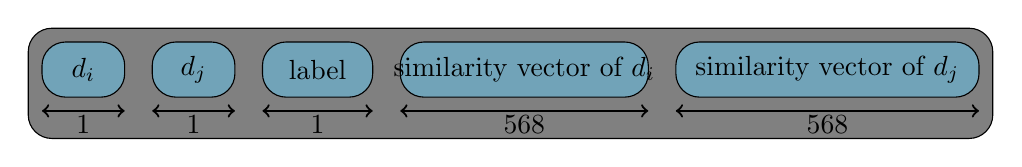
\begin{tikzpicture}[scale=.7]
\draw[rounded corners=3mm, fill=gray] (-0.25, 2.25) rectangle (17.25, 4.25);
\draw[rounded corners=3mm, fill=cyan!40!gray] (0, 3) rectangle (1.5, 4);
\node[inner sep=0pt] (di) at (0.75,3.5) {$d_i$};
\draw[rounded corners=3mm, fill=cyan!40!gray] (2, 3) rectangle (3.5, 4);
\node[inner sep=0pt] (dj) at (2.75,3.5) {$d_j$};
\draw[rounded corners=3mm, fill=cyan!40!gray] (4, 3) rectangle (6, 4);
\node[inner sep=0pt] (dj) at (5,3.5) {label};
\draw[rounded corners=3mm, fill=cyan!40!gray] (6.5, 3) rectangle (11, 4);
\node[inner sep=0pt] (dj) at (8.75,3.5) {similarity vector of $d_i$};
\draw[rounded corners=3mm, fill=cyan!40!gray] (11.5, 3) rectangle (17, 4);
\node[inner sep=0pt] (dj) at (14.25,3.5) {similarity vector of $d_j$};

\draw[<->, thick] (0, 2.75) -- (1.5, 2.75);
\draw[<->, thick] (2, 2.75) -- (3.5, 2.75);
\draw[<->, thick] (4, 2.75) -- (6, 2.75);
\draw[<->, thick] (6.5, 2.75) -- (11, 2.75);
\draw[<->, thick] (11.5, 2.75) -- (17, 2.75);

\node[inner sep=0pt] (dj) at (0.75,2.5) {1};
\node[inner sep=0pt] (dj) at (2.75,2.5) {1};
\node[inner sep=0pt] (dj) at (5,2.5) {1};
\node[inner sep=0pt] (dj) at (14.25,2.5) {568};
\node[inner sep=0pt] (dj) at (8.75,2.5) {568};
\end{tikzpicture}
\caption{Matrix scheme of tabular input data ($B$ matrix)}
\label{tableB}
\end{figure*}

\subsection{Dataset and features}\label{subsec2}
% This study utilizes the dataset introduced by Yu et al. in 2018~\cite{Yu2018}, comprising 568 approved small-molecule drugs. Each drug within the dataset exhibits at least one interaction with other drugs, resulting in a total of 21,351 Drug-Drug Interactions (DDIs). Notably, these interactions are further categorized into 16,757 enhancive DDIs and 4,594 degressive DDIs.
% Each drug in the dataset is uniquely characterized by two feature vectors:
% \begin{enumerate}
%     \item An 881-dimensional feature vector (Fstr) derived from PubChem chemical structure descriptors.
%     \item A 9149-dimensional feature vector (Fse) based on off-label side effects sourced from the OFFSIDES database~\cite{Tatonetti2012}.
% \end{enumerate}
% The elements in these vectors are binary, assigned a value of one if the corresponding side effect or chemical structure is reported or observed for the drug and zero otherwise.
% This dual-feature representation encapsulates both the structural attributes and off-label side effects of each drug, forming the foundational elements for subsequent analyses in our investigation.
This study utilizes the dataset introduced by Yu et al. in 2018~\cite{Yu2018}, comprising 568 approved small-molecule drugs. Each drug within the dataset exhibits at least one interaction with other drugs, resulting in a total of 21,351 Drug-Drug Interactions (DDIs). Notably, these interactions are further categorized into 16,757 enhancive DDIs and 4,594 degressive DDIs.
Each drug in the dataset is uniquely characterized by two feature vectors:
\begin{enumerate}
 \item An 881-dimensional feature vector ($F_{str}$) derived from PubChem chemical structure descriptors.
 \item A 9149-dimensional feature vector ($F_{se}$) based on off-label side effects sourced from the OFFSIDES database~\cite{Tatonetti2012}.
\end{enumerate} 
The elements in these vectors are binary, assigned a value of one if the corresponding side effect or chemical structure is reported or observed for the drug and zero otherwise. This dual-feature representation encapsulates each drug's structural attributes and off-label side effects, forming the foundational elements for subsequent analyses in this investigation.
\subsection{Data preparing}\label{subsec2}
Since the new drugs are isolated nodes in the interaction network, it is impossible to infer their potential interaction from topological information alone. Therefore, additional information, such as chemical structure or off-label side effects, is necessary and is referred to as a drug feature in machine learning. First, feature matrix data is prepared as input for machine learning methods, and then a deep learning model is devised and trained to predict potential interactions.
\subsection{Integration drug similarity matrices}
% Similarity Network Fusion (SNF) \cite{Wang2014} is a new computational method for data integration. Briefly, SNF combines many different types of features (such as chemical structure and off-label side effects, and more - clinical data, questionnaires, image data, etc.) for a given set of samples (e.g., drugs). SNF first constructs a sample similarity network for each of the data types and then iteratively integrates these
% networks using a novel network fusion method. Working in the sample network space allows SNF to avoid dealing with different scales, collection bias, and noise in different data types. Integrating data in a non-linear fashion allows SNF to take advantage of the common and complementary information in different data types. Figure 1 is a good visualization of SNF processes used in our method
% structure.
% In this section, similarity matrices of the chemical structure and the off-label side effects of drugs were integrated via the SNF method. The output of this integration is a new similarity matrix; Ssnf has dimensions of 568 × 568, and elements of Ssnf have a value between 0 and 1. To integrate the network similarity, the package of SNFPy, which is implemented in Python and is available at [40], is used.
SNF \cite{Wang2014} is a computational method for integrating diverse data types, such as chemical structure, off-label side effects, clinical data, questionnaires, and image data, for a given set of samples (e.g., drugs). SNF constructs sample similarity networks for each data type and iteratively integrates these networks using a novel fusion method. Operating in the sample network space enables SNF to handle different scales, collection bias, and noise across data types. By integrating data non-linearly, SNF leverages both common and complementary information. 
% Figure~\ref{figSNFCNN} illustrates the SNF process used in this study.
In this section, similarity matrices of the chemical structure and off-label side effects of drugs were integrated using the SNF method. The new similarity matrix ($S_{snf}$) output has dimensions of $568 \times 568$, with elements ranging from 0 to 1. The SNFPy~\cite{snfpy} package of  Python was used for network similarity integration.
\subsection{Input matrix format}
% At this stage, a matrix forms with $1139$ columns and $322056$ rows. Figure 2 shows the input data header, including the following columns:
% Drug pairs: Name of the drug i-th and the name of the drug j-th.
% Type of interaction: degressive (-1), enhancive (+1), and unknown (0).
% The similarity vector of the i-th drug from the Ssnf matrix has 568 elements.
% The similarity vector of the j-th drug from the Ssnf matrix has 568 elements.
% The data contains 568 drugs. The interaction of a drug with itself is meaningless. On the other hand, the drug pairs of ($d_i$, $d_j$) and ($d_j$, $d_i$) have the same label, while the corresponding similarity vectors of drugs in the B have been displaced, so these drug pairs are dual. Both dual augments the training data, increasing the model’s ability to have a better prediction. As a result, the matrix has $322056$ data samples or rows ($(568 × 568) - 568 = 322056$). According to the explanation, a matrix with dimensions of $322056 × 1139$ is formed to input into our model called the $B$ matrix.

% SNF processes \cite{Wang2014}: A detailed example of SNF steps. (a) An example representation of chemical structure feature and off-label side effect feature for the same set of drugs. (b) Drug-drug similarity matrices for each feature type. (c) Drug-drug similarity networks are equivalent to the drug-drug data. Nodes represent drugs, and edges represent drug pairwise similarities. (d) Network fusion by SNF iteratively updates each network with information from the other networks, making them more similar with each step. (e) The iterative network fusion results in convergence to the final fused network. The edge color indicates which data type has contributed to the given similarity.
A matrix is formed at this stage with $1139$ columns and $322056$ rows. Figure~\ref{tableB} displays the input data header, including two columns for drug pair names (the names of $d_i$ and $d_j$) and the type of interaction (degressive (-1), enhancive (+1), and unknown (0)). Each similarity vector from the Ssnf matrix for drug $i$ and drug $j$ has 568 elements.
The dataset comprises 568 drugs. However, interactions of a drug with itself are disregarded. Drug pairs ($d_i$, $d_j$) and ($d_j$, $d_i$) share the same label, augmenting the training data and improving prediction accuracy. Hence, the matrix has $322056$ data samples or rows ($(568 \times 568) - 568 = 322056$). Consequently, a matrix with dimensions of $322056 \times 1139$ forms the input for the model, referred to as the $B$ matrix.

SNF processes \cite{Wang2014}: A detailed example of SNF steps:
\begin{enumerate}
    \item Illustration of chemical structure and off-label side effect features for the same set of drugs.
\item Drug-drug similarity matrices for each feature type.
\item Drug-drug similarity networks correspond to the data, with nodes representing drugs and edges representing pairwise similarities.
\item Network fusion through SNF iteratively updates each network with information from the others, increasing their similarity.
\item Iterative network fusion converges to the final fused network, with edge color indicating the contributing data type.
\end{enumerate}
\subsection{Devising of Recommender System}
The data was meticulously prepared in the earlier stages to cater to various learning machines, by employing deep learning techniques. While positive and negative DDIs are labeled distinctly, the zero label does not denote the absence of interaction between a drug pair. Instead, it indicates that no interaction has been identified for that specific drug pair. The method of identifying pairs of non-interaction drugs is outlined in the next section. These drug pairs are then utilized as zero-labeled data in the subsequent training phase.
\subsection{Selecting model}
% We partitioned the rows of matrix $B$ to isolate instances of positive and negative interactions, resulting in a new matrix comprising $42,702$ drug pairs exhibiting degressive and enhancive interactions. This curated dataset served as the foundation for model training and selection, where a robust deep neural network model incorporating convolutional and fully connected layers is identified.

% The interaction data, denoted by positive and negative labels ($+1$ and $-1$), comprises feature vectors comprising $1136$ elements. Diverse models underwent consideration, and the chosen model underwent rigorous training in a $10$-fold CV procedure, employing $90$ percent of the data for training. Subsequently, the model’s performance was evaluated on the remaining $10$ percent of the data. Throughout the data split process, the dual drug pairs duals were considered. Acknowledging that drug pairs ($d_i$, $d_j$) and ($d_j$, $d_i$) lack biological distinctions, these pairs were consistently grouped in both training and testing sets, ensuring methodological integrity and preventing potential biases that could yield unfair results.


% After testing the different structures, the final deep neural network model is shown in Figure 3. This network has three layers of two-dimensional convolution. In the following, there are three fully connected convolution layers. The last layer has two outputs for predicting degressive or enhancive interaction. Convolution layers have 4-dimensions square filters with a Stride of 1. Each convolution layer also has a Rectified Linear Units (ReLU) activation function \cite{nair2010} as follows.
The matrix of $B$ as shown in Figure~\ref{tableB}, formed the basis for training a DNN model. Rows of $B$ are divided to isolate positive and negative interaction instances, creating a new matrix with $42,702$ drug pairs showing degressive and enhancive interactions. Interaction data, labeled as $+1$ and $-1$, comprises feature vectors of $1136$ elements. After considering various models, the selected one underwent a rigorous 10-fold CV. Drug pairs ($d_i$, $d_j$) and ($d_j$, $d_i$) were treated as dual identical to ensure methodological integrity. The final DNN model shown in Figure~\ref{CNNmodel} includes three 2D convolution layers followed by three fully connected layers, with the last layer predicting degressive or enhancive interactions. Convolution layers use 4-dimensional square filters with a Stride of 1 and ReLU activation function \cite{nair2010}.
\begin{figure}[htp]
    \centering
    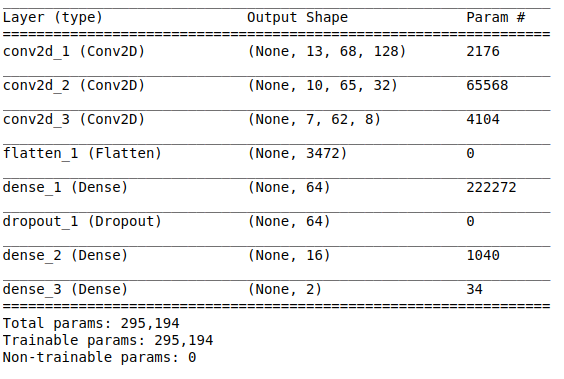
\includegraphics[width=8cm]{modelparameters}
    \caption{CNN model structure with Learnable parameters}
    \label{CNNmodel}
\end{figure}
% as follows.
% % , which is defined as the positive part of its argument:
% \begin{equation}
%     \text{ReLU}(x) = \max\{x,  0\}
% \end{equation}
% The convolution filters are $128$, $32$, and $8$, respectively. All connected layers have $64$, $16$, and $2$ nodes, respectively. The first two layers have the activation function of ReLU, and the last layer with two nodes has a Sigmoid activation function \cite{Hinton2012}, which is calculated as follows:
The convolution filters are sized at $128$, $32$, and $8$. The connected layers consist of $64$, $16$, and $2$ nodes, respectively. The first two layers utilize the ReLU activation function, while the final layer with two nodes uses the Sigmoid activation function \cite{Hinton2012}.
% , defined as follows:
% \begin{equation}
%     \text{Sigmoid}(x) =\frac{1}{1 + e^{-x} } 	
% \end{equation}	

% Convolution layers using a flattened layer connect to fully connected layers. The function of this layer is to transform a two-dimensional matrix into a one-dimensional vector. The output of this input layer of the first layer is fully connected. Also, between fully connected 64 and 16 nodes, one Dropout layer is used \cite{Srivastava2014} with a waste value of $0.2$. This value indicates that the network in this layer does not randomly consider $20$ percent of the features. This layer is used to prevent over-fitting of the model and forces the model to extract and use more features with more confidence for prediction. If some of them are removed, the algorithm’s prediction power either does not decrease or does not rely on a few specific features. 
% Our studies and trials have shown that two-dimensional convolution layers work better than their one-dimensional counterparts because, in this case, the filters can detect more drug similarities, and it is possible to extract more powerful Features. Therefore, the 1136-dimension feature vectors are transformed into matrices with dimensions of 17×16 times. Figure 4 shows the number of learnable weights for each layer. Also, the total number of weights is calculated, which indicates the general
% complexity of the model.
Convolution layers are followed by a flattened layer, which converts a 2-dimensional(2-D) matrix into a 1-D vector. The vector is fed into the first fully connected layer. Additionally, a Dropout layer with a dropout rate of $0.2$ is inserted between the fully connected layers of 64 and 16 nodes \cite{Srivastava2014}. This layer helps prevent overfitting by randomly ignoring $20$ percent of the features.

Experiments have demonstrated that two-dimensional convolution layers outperform their one-dimensional counterparts, as they can detect more drug similarities and extract more robust features. Thus, the 1136-dimensional feature vectors are transformed into matrices with dimensions of $17\times 16$.

The following settings are used in the construction of the convolution neural network:
\begin{enumerate}
    \item TensorFlow \cite{Abadi2016} (version 1.14.0) and KERAS~\cite{Keras} are used (version 2.2.5) packages to implement the neural network.
    \item The categorical-cross entropy loss function was considered an objective function for the neural network, which is generally used to train a classification network \cite{Ghosal_Edithal_Ekbal_Bhattacharyya_Chivukula_Tsatsaronis_2021, toda2019, giseop}.
    \item ADAM optimization \cite{Kingma2014} was used to manipulate the neural network weights to find a promising optimal (minimum) state of the loss function.
    \item The number of epochs was considered 5.
    \item A learning rate of $ 10^{-5}$ was used.
\end{enumerate}
\subsection{Hyper-parameters Optimization}
% Remember that the network’s hyper-parameters are not optimized, and the specified parameters are not necessarily at their best. There are two reasons for not optimizing hyper-parameters:
% 1) Model overfitting: If hyper-parameters changed to the best values, it is expected that the model will get better results on the present data, but there is no guarantee that the extracted features by the model are significant and work well when used in new cases. In this case, the so-called model is over-fitted and will be a negative point for the model.
% 2) Robustness: Optimal hyper-parameters give better results for the present data, but different drug similarities may be used in the future, or new data may be collected, and the present results may not be repeated. In this case, the model loses robustness and will not be accepted in the pharmaceutical and pharmacological community.
Note that the hyper-parameters of the network have not been optimized, so the specified parameters may not represent the best configuration. There are two reasons for not optimizing hyper-parameters:
\begin{enumerate}
    \item Model Overfitting: Optimizing hyper-parameters for the best performance on specific data may increase the risk of overfitting. While this can enhance the results, it does not ensure the learned features will generalize effectively to new unseen data. Overfitting diminishes the model’s utility in real-world scenarios.
    \item Robustness: While Optimal hyper-parameters yield better results on the current data, they may not generalize well for a new drug with outlier drug similarities in the future. A model that lacks robustness may fail to perform adequately when applied to novel scenarios, undermining its credibility and acceptance within the pharmaceutical and pharmacological community.
\end{enumerate}
While hyper-parameter optimization is a common step of model development, it must be approached cautiously to balance performance on current data with the model’s ability to generalize to unseen cases and maintain robustness over time.

%%%%%%%%%%%%%%%%%%%%%%%%%%%
The SNF-CNN method’s steps are presented in the form of Algorithm~\ref{algo1final}, and also Figure~\ref{figSNFCNN} shows the visual process which includes data preparation, model selection, non-DDI detection, and the final comprehensive recommender system.
\begin{algorithm}[!t]
\caption{Final model selection (SNF-CNN) pseudocode}\label{algo1final}
\begin{algorithmic}[1]
\Require Input: Drug pairs features (+1, -1, real 0)

~~~Features matrices of chemical and off-label 
% \Ensure $y = x^n$
\State Drug similarity calculation on feature matrices via cosine.
\State Integrate drug similarity matrices with the SNF method.
\State Built the input matrix of $B$.
\State Select known interactions and train the CNN.
\State Predict probable zeros using the model from step 4.
\State Select the known interactions from step 4 and zeros from the step 5 model to train a new CNN.
\State Predict on unknown drug pairs.
\Ensure Output: triple-class diagnostic model 
% \If{$n < 0$}
%         \State $X \Leftarrow 1 / x$
%         \State $N \Leftarrow -n$
% \Else
%         \State $X \Leftarrow x$
%         \State $N \Leftarrow n$
% \EndIf
% \While{$N \neq 0$}
%         \If{$N$ is even}
%             \State $X \Leftarrow X \times X$
%             \State $N \Leftarrow N / 2$
%         \Else[$N$ is odd]
%             \State $y \Leftarrow y \times X$
%             \State $N \Leftarrow N - 1$
%         \EndIf
% \EndWhile
\end{algorithmic}
\end{algorithm}
\section{Implementation}\label{sec4}

\subsection{two-classes model’s training trend}
The training data for the two-class model is generated by randomly selecting $90\%$ of the enhancive and degressive interactions. The remaining $10\%$ is allocated for testing. In the training phase, the model is selected, and certain hyper-parameters for instance, the number of epochs are determined by $5$. The selection process of $5$ is elaborated in the supplementary file.
\begin{figure*}[!t]%
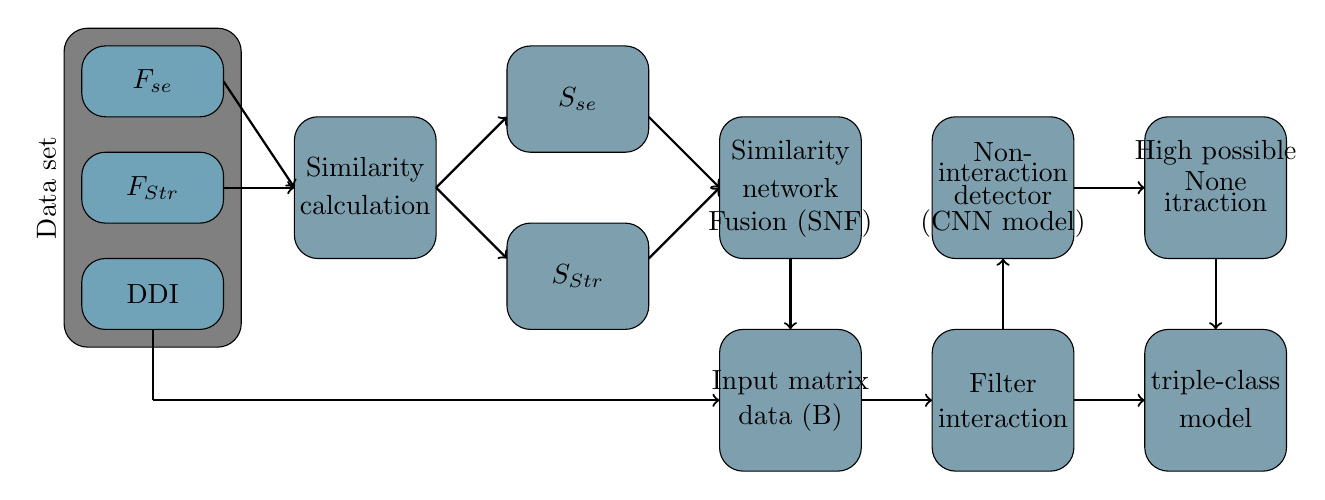
\begin{tikzpicture}[scale=.9]
% Define the nodes
\node[rotate=90] (ddi) at (-0.5,2) {Data set};
\draw[rounded corners=3mm, fill=gray] (-0.25, -0.25) rectangle (2.25, 4.25);
\draw[rounded corners=3mm, fill=cyan!40!gray] (0, 0) rectangle (2, 1);
\draw[rounded corners=3mm, fill=cyan!40!gray] (0, 1.5) rectangle (2, 2.5);
\draw[rounded corners=3mm, fill=cyan!40!gray] (0, 3) rectangle (2, 4);
\node[inner sep=0pt] (ddi) at (1,0.5) {DDI};
\node[inner sep=0pt] (fs) at (1,2) {$F_{Str}$};
\node[inner sep=0pt] (fo) at (1,3.5) {$F_{se}$};
\draw[rounded corners=3mm, fill=cyan!30!gray] (3, 1) rectangle (5, 3);
\node[inner sep=0pt] (conv2d_1) at (4,2.25) {\text{Similarity}};
\node[inner sep=0pt] (conv2d_1) at (4,1.75) {\text{calculation}};
\draw[rounded corners=3mm, fill=cyan!30!gray] (6, 0) rectangle (8, 1.5);
\node[inner sep=0pt] (conv2d_1) at (7,0.75) {$S_{Str}$};
\draw[rounded corners=3mm, fill=cyan!30!gray] (6, 2.5) rectangle (8, 4);
\node[inner sep=0pt] (conv2d_1) at (7,3.25) {$S_{se}$};
\draw[rounded corners=3mm, fill=cyan!30!gray] (9, 1) rectangle (11, 3);
\node[inner sep=0pt] (conv2d_1) at (10,2.5) {\text{Similarity}};
\node[inner sep=0pt] (conv2d_1) at (10,2) {\text{network}};
\node[inner sep=0pt] (conv2d_1) at (10,1.5) {\text{Fusion (SNF)}};
\draw[rounded corners=3mm, fill=cyan!30!gray] (9, -2) rectangle (11, 0);
\node[inner sep=0pt] (conv2d_1) at (10,-0.75) {\text{Input matrix}};
\node[inner sep=0pt] (conv2d_1) at (10,-1.25) {\text{data (B)}};
\draw[rounded corners=3mm, fill=cyan!30!gray] (12, -2) rectangle (14, 0);
\node[inner sep=0pt] (conv2d_1) at (13,-0.75) {\text{Filter}};
\node[inner sep=0pt] (conv2d_1) at (13,-1.25) {\text{interaction}};
\draw[rounded corners=3mm, fill=cyan!30!gray] (12, 1) rectangle (14, 3);
\node[inner sep=0pt] (conv2d_1) at (13,2.5) {\text{Non-}};
\node[inner sep=0pt] (conv2d_1) at (13,2.22) {\text{interaction}};
\node[inner sep=0pt] (conv2d_1) at (13,1.9) {\text{detector}};
\node[inner sep=0pt] (conv2d_1) at (13,1.5) {\text{(CNN model)}};
\draw[rounded corners=3mm, fill=cyan!30!gray] (15, -2) rectangle (17, 0);
\node[inner sep=0pt] (conv2d_1) at (16,-0.75) {\text{triple-class}};
\node[inner sep=0pt] (conv2d_1) at (16,-1.25) {\text{model}};
\draw[rounded corners=3mm, fill=cyan!30!gray] (15, 1) rectangle (17, 3);
\node[inner sep=0pt] (conv2d_1) at (16,2.5) {\text{High possible}};
\node[inner sep=0pt] (conv2d_1) at (16,2.1) {\text{None}};
\node[inner sep=0pt] (conv2d_1) at (16,1.8) {\text{itraction}};
% \node[inner sep=0pt] (x2) at (9.5,0.5)
%     {\text{{$\boldsymbol{x}(k+2)$}}};
\draw[-, thick] (1, 0) -- (1, -1);  
\draw[->, thick] (1, -1) -- (9, -1); 
\draw[->, thick] (2, 2) -- (3, 2); 
\draw[->, thick] (2, 3.5) -- (3, 2); 
\draw[->, thick] (5, 2) -- (6, 3); 
\draw[->, thick] (5, 2) -- (6, 1); 
\draw[->, thick] (8, 1) -- (9, 2); 
\draw[->, thick] (8, 3) -- (9, 2);
\draw[->, thick] (10, 1) -- (10, 0);
\draw[->, thick] (11, -1) -- (12, -1);
\draw[->, thick] (14, -1) -- (15, -1);
\draw[->, thick] (14, 2) -- (15, 2);
\draw[->, thick] (13, 0) -- (13, 1);
\draw[->, thick] (16, 1) -- (16, 0);
\end{tikzpicture}
\caption{Flowchart of the comprehensive DDI prediction from raw data to the end model (SNF-CNN)}
\label{figSNFCNN}
\end{figure*}
\subsection{Reliability of the two-classes model}
The proposed model is examined in the 10-fold CV from three perspectives:
\begin{enumerate}
    \item Model Resolution: In a 10-fold CV, the model obtained AUC = $0.97$, AUPR = $0.93$ for degressive interactions, and AUC = $0.97$, AUPR = $0.99$ for enhancive interactions. These results indicate the high resolution and detection power of the selected model.

\begin{table}
% \tabcolsep=0pt%%
\begin{tabular}{|c|c|c|c|c|}
% \toprule%
 \hline
         & Precision& Recall& F-measure& Support
\\\hline
        Degressive&0.94&0.83&0.88&3902\\
Enhancive&0.95&0.99&0.97&
3902\\
% \botrule
\hline
\end{tabular}
\caption{Interaction type classification report.}
\label{t2}
\end{table}
Table~\ref{t2} presents an example result of the implemented model, showcasing its precision, recall, and F-measure in detecting the different types of interactions. As per Table~\ref{t2}, the model achieved $95\%$ precision for detecting enhancive interactions and $94\%$ for degressive interactions, with recall rates of $99\%$ and $83\%$, respectively. Additionally, the F-measure stands at $97\%$ for enhancive interactions and $88\%$ for degressive interactions. The model’s superior ability to detect degressive interactions stems from their higher prevalence, with a ratio of approximately $4$ degressive interactions to $1$ enhancive interaction.
\item Variance: The confidence interval for the reported values with a reliability coefficient above $95$ percent was narrow and close to each other. Out of four reported confidence interval values, three values were less than $\pm0.002$, and only the AUPR was in the range of $\pm0.005$ for the degressive interaction. The low variance of the model is evidence robustness of the proposed model.
\item Separability: By plotting the output probability distribution diagram, as shown in Figure~\ref{preddensity}, values $+1$ and $-1$ are well separated, and probability distribution degressive and enhancive have a smaller intersection.
\begin{figure}[htp]
    \centering
    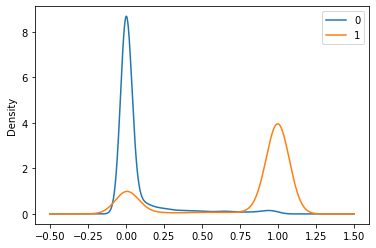
\includegraphics[scale=.5]{PredictonDensity(-1,+1)}
    \caption{Probability density distribution of degressive and enhancive. Here, 0 is the same as the $-1$ label (for technical reasons), and $1$ is the same as $+1$.}
    \label{preddensity}
\end{figure}
\end{enumerate}  
\subsection{Detecting of non-interaction drug pairs}
% In the previous step, a high-precision, robust, and accurate model has been presented to detect drug pairs’ potential interactions for both degressive and enhancive.
% Therefore, this model has the ability to detect non-interactions (real zeros) as follows. If drug pairs are unlikely to interact, then those drug pairs are likely to be real zeros.
% According to this hypothesis, the model was used to predict all unknown drug pairs (zeros). Unknown drug pairs include 270,000 drug pairs. We consider drug pairs as non-interacting drug pairs in the model’s output if the enhancive and degressive probability are less than 0.4 and 0.4. Among the unlabeled data, about 65,000 drug pairs had these conditions. These drug pairs are candidates for non-interaction. Due to the model’s high accuracy, the low variance of results, and the model’s high resolution, we consider these pairs non-interaction drug pairs. 
In the previous step, a precise model was introduced to detect potential interactions between drug pairs, both enhancive and degressive interactions. This model can also identify non-interactions or 'real zeros'. If a drug pair shows little likelihood of interaction, it is classified as a 'real zero'.

To apply this rule, the model was used to predict interactions among $270,000$ drug pairs with unknown labels. Pairs with both enhancive and degressive probabilities below 0.4 were classified as non-interaction. Approximately $65,000$ pairs met these criteria and were considered candidates for non-interaction. Given the model’s accuracy, consistent results, and high resolution, these pairs are confidently considered as non-interactions.

\subsection{Triple-class model training trend}\label{subsec2}
This section focuses on selecting and training models using both known interactions and potential non-interaction candidates. Non-interaction candidate drug pairs are treated as real zeros. The recommender system introduced in the previous section is utilized for the final model.

As detailed previously, the B matrix rows with $+1$ and $-1$ interactions are divided into ten parts. From the $65,000$ non-interaction candidate drug pairs, $30,000$ are randomly selected, ensuring each pair and its dual are included. The zero group is split into ten parts, aligned with the $+1$s and $-1$s. These parts are merged, resulting in a dataset of approximately $72,702$ drug pairs evenly divided and suitable for training and testing the final recommender system.
% First, the B matrix rows containing the +1 and -1 interactions are separated according to the previously detailed procedure and placed in 10 parts. Then, 30,000 non-interacting candidate drug pairs were randomly selected from 65,000 drug pairs. In the chosen drug pairs, the drug pairs and the dual of them must be non-interaction candidates. The zeros group is randomly divided into ten parts, so each drug pair and the dual are in the same batch. Then, ten parts of zeros are merged with ten parts of pre-prepared +1s and -1s.
% The data set contains approximately 72,702 drug pairs, divided into relatively equal parts, and is ready to use in the training and testing of the final recommender system.

% The all interactions dataset (enhancive, degressive) is divided into ten parts. 
% One part is considered as the testing set and the rest is the training data.
% All the zeros in the previous step are divided into ten parts and are combined into the subset data subsets.
Then, the previous model is trained and validated in a 10-fold CV procedure for triple-class prediction. Only the output layer is adapted to have three categorical outputs. The number of epochs was determined by $9$. The process of selecting $9$ is elaborated in the supplementary file.
% Figure 8 shows the training process. The model’s accuracy on training data increases steadily with the increase of epochs. Still, the model after epoch 9 reduces a constant and decreases the accuracy a little for testing data.
\section{Discussion}\label{sec5}
% Each model feature setting and data set needs its validation process. According to the type of problem and the methods, we use two types of 10-fold CV to select the most proper model and validate the results of the chosen model. The metrics that are used in validation are described below.
Every combination of model and feature set has to undergo a validation process. Depending on the nature of the problem and the chosen methodology, two variants of 10-fold CV were employed to ascertain the most suitable model and validate its results. The selection and evaluation of models were conducted with meticulous attention to the specific metrics detailed below.
\subsection{Evaluation criteria for the final triple-class model}\label{subsec2}
% In this study, we classify drug pairs into three classes, according to the type of interaction or non-interaction, to compare the method performance with other existing methods, four measurement criteria, F- measure, accuracy, Area Under Roc Curve (AUC), and Area Under Precision-Recall curve (AUPR) are used. We should use a confusion matrix to define these criteria, as Table~\ref{tab3} demonstrates.
% Table~\ref{tab3} shows the confusion matrix for the triple class case. In this mode, we must redefine the definitions of TP, TF, TN, and TP, as well as accuracy, precision, recall, and F-measure.
In this study, drug pairs are classified into three classes based on interaction type for performance comparison. Methods are evaluated via adapted AUC and AUPR for the triple-class model using the confusion matrix table in the supplementary file with detail.
% ~\ref{tab3}). 
% The confusion matrix for the triple-class case requires the redefinition of TP, TF, TN, and FP, as well as accuracy, precision, recall, and F-measure.
% \begin{table*}[t]
% \tabcolsep=0pt%%
% \begin{tabular*}{\textwidth}{@{\extracolsep{\fill}}lcccccc@{\extracolsep{\fill}}}
% \toprule%
%  % \hline
%          & Actual Enhancive & Actual Degressive & Actual Non-interaction\\\hline
%         Predicted Enhancive & $cell_{1}:T_{Enh}$ & $cell_2:F_{Enh}$ & $Cell_3:F_{Enh}$ \\
%         Predicted Degressive & $cell_4:F_{Deg}$& $cell_5:T_{Deg}$&$cell_6:F_{Deg}$ \\
%         Predicted Non-interaction & $cell_7:F_{Non-Int}$&$cell_8:F_{Non-Int}$&$cell9:T_{Non-Int}$
%   \\
% \botrule
% \end{tabular*}
% \caption{The confusion matrix and relevant evaluation index for predicting triple-class whose cell
% names start with T (True). The main diagonal amounts of the matrix show correct predictions for
% each class. The other cells show drug pairs classified by mistake whose cell names
% start with F (False)..}
% \label{tab3}
% \end{table*}
% % \begin{table}[]
% %     \centering
% %     \begin{tabular}{|c|c|c|c|}
% %     \hline
% %          & Actual Enhancive & Actual Degressive & Actual Non-interaction\\\hline
% %         Predicted Enhancive & $cell_{1}:T_{Enh}$ & $cell_2:F_{Enh}$ & $Cell_3:F_{Enh}$ \\
% %         Predicted Degressive & $cell_4:F_{Deg}$& $cell_5:T_{Deg}$&$cell_6:F_{Deg}$ \\
% %         Predicted Non-interaction & $cell_7:F_{Non-Int}$&$cell_8:F_{Non-Int}$&$cell9:T_{Non-Int}$\\\hline
% %     \end{tabular}
% %     \caption{The confusion matrix and relevant evaluation index for predicting triple-class whose cell
% % names start with T (True). The main diagonal amounts of the matrix show correct predictions for
% % each class. The other cells show drug pairs classified by mistake whose cell names
% % start with F (False).
% % }
% %     \label{tab3}
% % \end{table}
% $\text{Accuracy}_{(enh/deg/nonInt)}$: The fraction of all correct predictions (TPs) to all predictions.
% \begin{equation}
%    \text{Accuracy}=\frac{\text{All correctly predicted} (cell_1 + cell_5 + cell_9 )}{\text{Summation all nine cells} (\sum_{i=1}^9 cell_i)} 
% \end{equation}
% Based on Table~\ref{tab3}, TP, TF, TN, and TP will be defined in Table~\ref{tab4} for the triple-class scenario.
% The other three evaluation criteria for each class are defined as follows:

% Precision: The ratio of correct predicted ($TP_{Enh/Deg/Non-Int}$) interactions among all predicted (Enh/Deg/Non-Int) interactions.
% \begin{equation}
% \begin{aligned}
%     \text{Precision}_{(Enh/Deg/Non-Int)}\\=\frac{TP_{(Enh/Deg/Non-Int)}}{TP_{(Enh/Deg/Non-Int)}+ FP_{(Enh/Deg/Non-Int)}}
%     \end{aligned}
% \end{equation}
% \begin{table*}[t]
% \tabcolsep=0pt%%
% \begin{tabular*}{\textwidth}{@{\extracolsep{\fill}}lcccccc@{\extracolsep{\fill}}}
% \toprule%
%  % \hline
%          Enhancive&Degressive&Non-interaction\\\hline
% $TP = cell_1$&$TP = cell_5$&$TP = cell_9$\\
% $FP = cell_2 + cell_3$&$FP = cell_4 + cell_6$&
% $FP = cell_7 + cell_8$\\
% $FN = cell_4 + cell_7$&$FN = cell_2 + cell_8$&
% $FN = cell_3 + cell_6$\\
% $TN = cell_5 + cell_6 + cell_8 + cell_9$&
% $TN = cell_1 + cell_3 + cell_7 + cell_9$&
% $TN = cell_1 + cell_2 + cell_4 + cell_5$
%   \\
% \botrule
% \end{tabular*}
% \caption{The new definition of TP, TN, FP, and FN in the triple class mod.}
% \label{tab4}
% \end{table*}
% Recall: The ratio of correct predicted ($TP_{Enh/Deg/Non-Int}$) interactions among all true (Enh/Deg/Non-Int) interactions.
% \begin{equation}
% \begin{aligned}
%     \text{Recall}_{(Enh/Deg/Non-Int)}\\=\frac{TP_{(Enh/Deg/Non-Int)}}{TP_{(Enh/Deg/Non-Int)}+ FN_{(Enh/Deg/Non-Int)}}\end{aligned}\end{equation}  				
% Precision and recall for each class have a trade-off; Therefore, the F-measure can show the resolution ability of the model in each class.
% F-measure: The geometric mean of precision and recall in three- classes:
% \begin{equation}
% \begin{aligned}
%     \text{F-measure}_{(Enh/Deg/Non-Int)} =\\ \frac{2 \times \text{Precision}_{(Enh/Deg/Non-Int)} \times \text{Recall}_{(Enh/Deg/Non-Int)}}{ \text{Precision}_{(Enh/Deg/Non-Int)} + \text{Recall}_{(Enh/Deg/Non-Int)}}\end{aligned}\end{equation}
% Also, methods were evaluated via modified AUC and AUPR for the triple-class model.
\subsection{Comparison of results}\label{subsec2}
The binary interaction type detection model is developed and trained following the validation procedure outlined in the previous section. Subsequently, the final triple-class model is introduced, utilizing the most probable non-interactions as zeros. The SNF-CNN model undergoes evaluation through a 10-fold CV to assess its robustness and efficiency. In this section, the results of the SNF-CNN model are compared with those of other methods, and the findings are discussed.
\begin{table}[t]
% \tabcolsep=0pt%
\begin{tabular}{|c|c|c|c|c|}
% \toprule%
 \hline
         &Precision&Recall&F-measure&Support\\\hline
Enhancive&0.88&0.84&0.86&850\\
Non-interaction&0.96&0.95&0.96&3000\\
Degressive&0.95&0.97&0.96&3052\\
% Macro Avg&0.93&0.92&0.93&0.95&6902\\
% Weighted Avg&0.95&0.95&0.95&0.95&6902
  % \\
% \botrule
 \hline
\end{tabular}
\caption{triple-class interaction classification report.}
\label{tab5}
\end{table}
% \begin{table}[]
%     \centering
%     \begin{tabular}{|c|c|c|c|c|c|}
%     \hline
% &Precision&Recall&F-measure&Accuracy&Support\\\hline
% Enhancive&0.88&0.84&0.86&&850\\
% Non-interaction&0.96&0.95&0.96&&3000\\
% Degressive&0.95&0.97&0.96&&3052\\
% Macro Avg&0.93&0.92&0.93&0.95&6902\\
% Weighted Avg&0.95&0.95&0.95&0.95&6902\\\hline
%     \end{tabular}
%     \caption{triple-class interaction classification report}
%     \label{tab5}
% \end{table}
In Table~\ref{tab5} the triple-classes interaction classification is displayed. In this implementation, the precision of the model in detecting degressive interactions, non-interactions, and enhancive interactions are $95\%$, $96\%$, and $88\%$, respectively. The recalls are $97\%$, $95\%$, and $84\%$, respectively, and F-measures are $96\%$, $96\%$, and $86\%$. The model power in the triple-classes mode decreases slightly compared to the two-classes mode, which can be due to two reasons:
\begin{enumerate}
    \item The triple-class mode is more difficult than the two-classes mode.
    \item The suggested non-interactions or zeros are not necessarily real or pharmacologically proven, so some disturbance is possible.
\end{enumerate}
For the above reasons, a reduction in the detection ability of the triple-class model was expected.
\begin{table}[]
    \centering
    \begin{tabular}{|c|c|c|}
    \hline
         &AUC&AUPR\\\hline
Degressive&0.9747 ± 0.0033&0.9666 ± 0.0045\\
Enhancive&0.9686 ± 0.0028&0.8221 ± 0.0184\\
Non-interaction&0.9714 ± 0.0040&0.9480 ± 0.0083\\\hline
    \end{tabular}
    \caption{Results of SNF-CNN algorithm in predicting three- classes based on AUC and AUPR criteria and their confidence interval}
    \label{tab6}
\end{table}
Since the previous three- classes of DDI models reported AUC and AUPR for comparison, the SNF-CNN results (Table~\ref{tab6}) are presented based on these criteria, including the error margin of a $95\%$ confidence interval. The small margin of the SNF-CNN in the 10-fold CV underscores the robustness and reliability of the proposed algorithm. 
% the SNF-CNN results, shown in Table~\ref{tab6}, are reported based on these two criteria. Also, the margin of error with the $95\%$ confidence interval is reported in Table~\ref{tab6}. The algorithm results have a small margin in the 10-fold CV, which shows the robustness and reliability of the proposed algorithm.
\begin{table}[]
    \centering
    \begin{tabular}{|c|c|c|}
         \hline
&AUC&AUPR\\\hline
SNF-CNN&0.971&0.912\\
BRSNMF~\cite{Shi2019}&0.805&0.644\\
Semi-NMF~\cite{lesly2018} &0.796&0.579\\
TMFUF~\cite{Shi2018}&0.842&0.526\\\hline
    \end{tabular}
    \caption{Comparison of the results of triple-class prediction algorithms based on criteria AUC and AUPR}
    \label{tab7}
\end{table}
Table~\ref{tab7} compares the SNF-CNN result with other existing triple-classes algorithms. The proposed algorithm exhibits a notable performance improvement compared to the state-of-the-art algorithms in addressing the ternary problem, showcasing its competitive performance.
\subsection{Conclusions}
% Existing machine learning approaches can detect potential drug interactions using large-scale data before taking the drug. However, they cannot predict comprehensive triple-class DDIs, including degressive and enhancive interactions. It is more informative to clarify if a drug pair has an enhancive DDI or a degressive DDI, or even non-DDI than to recognize a drug pair and whether or not it has a DDI. Without considering the pharmacological changes caused by DDIs, most existing approaches only report two-classes predictions. In addition, not only the occurrence of degressive and enhancive DDIs is not random, but it also represents a piece of information about the major behaviors of those two drugs. None of the existing approaches investigate and consider this intrinsically important property of interactions when treating complex diseases [34].
% In this work, after representing comprehensive DDI data and drug features, we used the template of recommender systems to design a novel algorithm. Although the prediction obtained by our algorithm was inspiring, overall performance could still be improved. DDIs are predicted incorrectly. T were investigated to prove the algorithm in practice. We checked the model prediction case-by-case in the DrugBank database’s latest version. Observations and investigations led to the discovery of three reasons for wrong predictions, all of them related to differences between versions 4 and 5 of the DrugBank:
% \begin{enumerate}
%     \item Removed interactions in DrugBank version 5. Data was precisely labeled in DrugBanck version 4, which is no longer labeled as such in version 5. For example, the old version of DrugBank version 4 records that Apraclonidine (DB00964) (also known as iopidine, is a sympathomimetic used in glaucoma therapy.) increases the atrioventricular blocking activities of Alprenolol (DB00866) and Bevantolol (DB01295), while version 5 removes them. This represents a problem for new research as data shows no interaction.
%     \item Drug Pairs labeled as non-DDIs. Some drug pairs are labeled as non-DDIs in the DrugBank version 4 drug and are reported as DDIs in version 5. For example, the pair of Valrubicin (DB00385) and Cyclosporine (DB00091), as well as the pair of Ergocalciferol (DB00153) and Calcitriol (DB00136) in the newer version of DrugBank, reports Valrubicin (bladder cancer treatment drug) Increases the activity of the nephrotoxic drug Cyclosporine (A drug that suppresses the immune system with a special action on T-lymphocytes), while the combined therapy of Calcitriol and Ergocalciferol increases the risk or severity of adverse effects in the multiple-drug therapy.
%     \item Altering DDIs’ types labeled as enhancive DDIs in DrugBank version 4 are labeled as degressive DDIs in version 5, and vice versa. 
% \end{enumerate}
% We expect that the SNF-CNN approach will achieve better results in DDI prediction with a better dataset with less missed or false information about drug pairs. For future research, it is recommended that drugs and their features be collected from the latest version of DrugBank.

% triple-class data is an attempt to improve expression and problem-solving over two-classes data. However, three- classes of data do not have sufficient biological significance and provide limited biological information. This means that predicting the type of DDI can be useful, but it is unclear at what stage of the pharmacokinetic or pharmacodynamic stages this DDI occurred. Therefore, collecting datasets with degressive and enhancive labels from each pharmacokinetic and pharmacodynamic step is suggested. More meaningful pharmacology and machine learning models may be designed and built in this case. Results from these models will be more important to pharmacists and will be more useful for further steps in human health aim.

% As future work, authors are also evaluating the possibility of extending the research by combining the results here presented with the results achieved within the Smart4Health project regarding pharmacogenomics for personalized health [c] to study DDI mechanisms in specific patient profiles and contribute to the development of personalized treatment schemes.
% Contemporary machine learning methodologies have demonstrated efficacy in detecting potential drug interactions using expansive datasets prior to drug administration. However, their ability to predict comprehensive triple-class Drug-Drug Interactions (DDIs), encompassing degressive and enhancive interactions, remains limited. It is imperative to discern not only the presence of a DDI between drug pairs but also to elucidate whether the interaction is enhancive, degressive, or non-existent. Regrettably, most existing approaches overlook the pharmacological alterations induced by DDIs, consequently restricting their predictions to binary classifications. Moreover, the non-random occurrence of degressive and enhancive DDIs not only imparts crucial information regarding the behavioral dynamics of the involved drugs but also underscores the inadequacy of current methodologies in addressing this nuanced aspect of complex diseases.
Modern machine learning methods effectively identify potential drug interactions using large datasets but struggle with comprehensive triple-class DDIs, including degressive, enhancive, and non-interactions. Current approaches often focus solely on binary classifications, overlooking pharmacological nuances. The distinct patterns of degressive and enhancive DDIs highlight the limitations of existing methodologies in capturing the complexities of drug interactions and disease dynamics.

This study aimed to fill this gap by utilizing extensive DDI data and drug features to create a novel algorithm inspired by recommender systems. While the proposed algorithm showed promising performance, there is still room for improvement, as indicated by false DDI predictions upon closer examination. A detailed investigation into model predictions, conducted through a case-by-case analysis of the latest versions of the DrugBank database, revealed three main reasons for erroneous predictions, all stemming from differences between DrugBank versions $4$ and $5$.
% In this study, we endeavored to address this gap by leveraging comprehensive DDI data and drug features to devise a novel algorithm inspired by recommender systems. While the performance of our algorithm yielded promising results, there remains room for enhancement, as evidenced by inaccuracies in DDI predictions upon scrutiny. A meticulous investigation into model predictions, undertaken through a case-by-case examination of the DrugBank database’s latest version, unveiled three primary reasons for erroneous predictions, all of which are attributable to disparities between versions $4$ and $5$ of DrugBank:
\begin{enumerate}
\item Removal of interactions in DrugBank version $5$, leading to discrepancies in labeled data compared to version $4$.
\item Inconsistencies in DDI labeling between DrugBank versions $4$ and $5$, resulting in misclassification of certain drug pairs.
\item Alterations in classifying DDIs between enhancive and degressive types between DrugBank versions $4$ and $5$.
\end{enumerate}
% We anticipate that the SNF-CNN approach will yield superior results in DDI prediction with an improved dataset that mitigates the prevalence of erroneous or missing information pertaining to drug pairs. For future research endeavors, it is imperative to procure drug-related data from the most recent version of DrugBank.
% While the transition from two-classes to triple-class data constitutes an effort to enhance representation and problem-solving capabilities, it is acknowledged that triple-class data may not inherently possess sufficient biological significance or provide comprehensive biological insights. Consequently, while predicting the type of DDI is undoubtedly beneficial, it remains ambiguous at which stage of the pharmacokinetic or pharmacodynamic processes these interactions manifest. To address this limitation, the collection of datasets featuring degressive and enhancive labels across each pharmacokinetic and pharmacodynamic step is recommended. Such datasets hold promise for facilitating the development of more nuanced pharmacological models, thereby furnishing pharmacists with invaluable insights and paving the way for advancements in human health objectives.
The SNF-CNN approach shows promising results that can deliver superior DDI predictions with an improved dataset, minimizing erroneous or missing information on drug pairs. Future research should prioritize acquiring drug-related data from the latest DrugBank version.

While transitioning from two-classes to triple-classes data aims to enhance representation and problem-solving capabilities, it is recognized that triple-classes data may not inherently provide sufficient biological insights. Therefore, collecting datasets featuring degressive and enhancive labels across pharmacokinetics and pharmacodynamics is recommended. These datasets hold promise for developing nuanced pharmacological models, offering valuable insights for pharmacists and advancing human health objectives.

As a prospect for future research, the authors are investigating potential synergies between the findings presented here and those from the Smart4Health project’s pharmacogenomics investigations for personalized health. This collaborative effort aims to understand DDI mechanisms across patient profiles, contributing to personalized treatment regimens.
\section{Funding}
This work was partially funded by the European Union’s Horizon 2020 research and innovation program in the scope of the Smart4Health under grant agreement No 826117 and by the Portuguese FCT program, Center of Technology and Systems (CTS) UIDB/00066/2020 / UIDP/00066/2020.
% \subsection{This is an example for second level head - subsection head}\label{subsec2}
% \subsubsection{This is an example for third level head - subsubsection head}\label{subsubsec2}
% Lorem ipsum dolor sit amet, consectetur adipiscing elit, sed do eiusmod tempor incididunt ut labore et dolore magna aliqua. Ut enim ad minim veniam, quis nostrud exercitation ullamco laboris nisi ut aliquip ex ea commodo consequat. Duis aute irure dolor in reprehenderit in voluptate velit esse cillum dolore eu fugiat nulla pariatur. Excepteur sint occaecat cupidatat non proident, sunt in culpa qui officia deserunt mollit anim id est laborum.
% \paragraph{This is an example for fourth level head - paragraph head}

% Lorem ipsum dolor sit amet, consectetur adipiscing elit, sed do eiusmod tempor incididunt ut labore et dolore magna aliqua. Ut enim ad minim veniam, quis nostrud exercitation ullamco laboris nisi ut aliquip ex ea commodo consequat. Duis aute irure dolor in reprehenderit in voluptate velit esse cillum dolore eu fugiat nulla pariatur. Excepteur sint occaecat cupidatat non proident, sunt in culpa qui officia deserunt mollit anim id est laborum.
% \section{Equations}\label{sec4}
% Equations in \LaTeX{} can either be inline or set as display equations. For
% inline equations use the \verb+$...$+ commands. Eg: the equation
% $H\psi = E \psi$ is written via the command \verb+$H \psi = E \psi$+.

% For display equations (with auto generated equation numbers)
% one can use the equation or eqnarray environments:
% \begin{equation}
% \|\tilde{X}(k)\|^2 \leq\frac{\sum\limits_{i=1}^{p}\left\|\tilde{Y}_i(k)\right\|^2+\sum\limits_{j=1}^{q}\left\|\tilde{Z}_j(k)\right\|^2 }{p+q},\label{eq1}
% \end{equation}
% where,
% \begin{align}
% D_\mu &=  \partial_\mu - ig \frac{\lambda^a}{2} A^a_\mu \nonumber \\
% F^a_{\mu\nu} &= \partial_\mu A^a_\nu - \partial_\nu A^a_\mu + g f^{abc} A^b_\mu A^a_\nu.\label{eq2}
% \end{align}
% Notice the use of \verb+\nonumber+ in the align environment at the end
% of each line, except the last, so as not to produce equation numbers on
% lines where no equation numbers are required. The \verb+\label{}+ command
% should only be used at the last line of an align environment where
% \verb+\nonumber+ is not used.
% \begin{equation}
% Y_\infty = \left( \frac{m}{\textrm{GeV}} \right)^{-3}
%     \left[ 1 + \frac{3 \ln(m/\textrm{GeV})}{15}
%     + \frac{\ln(c_2/5)}{15} \right].
% \end{equation}
% The class file also supports the use of \verb+\mathbb{}+, \verb+\mathscr{}+ and
% \verb+\mathcal{}+ commands. As such \verb+\mathbb{R}+, \verb+\mathscr{R}+
% and \verb+\mathcal{R}+ produces $\mathbb{R}$, $\mathscr{R}$ and $\mathcal{R}$
% respectively (refer Subsubsection~\ref{subsubsec3}).
% Lorem ipsum dolor sit amet, consectetur adipiscing elit, sed do
% eiusmod tempor incididunt ut labore et dolore magna aliqua. Ut enim ad minim veniam, quis nostrud exercitation ullamco laboris nisi ut aliquip ex ea commodo consequat. Duis aute irure dolor in reprehenderit in voluptate velit esse cillum dolore eu fugiat nulla pariatur. Excepteur sint occaecat cupidatat non proident, sunt in culpa qui officia deserunt mollit anim id est laborum. Lorem ipsum dolor sit amet, consectetur adipiscing elit, sed do
% eiusmod tempor incididunt ut labore et dolore magna aliqua. Ut enim ad minim veniam, quis nostrud exercitation ullamco laboris nisi ut aliquip ex ea commodo consequat. Duis aute irure dolor in reprehenderit in voluptate velit esse cillum dolore eu fugiat nulla pariatur. Excepteur sint occaecat cupidatat non proident, sunt in culpa qui officia deserunt mollit anim id est laborum. 
% Lorem ipsum dolor sit amet, consectetur adipiscing elit, sed do
% eiusmod tempor incididunt ut labore et dolore magna aliqua. Ut enim ad minim veniam, quis nostrud exercitation ullamco laboris nisi ut aliquip ex ea commodo consequat. 
% \section{Tables}\label{sec5}

% Tables can be inserted via the normal table and tabular environment. To put
% footnotes inside tables one has to Lorem ipsum dolor sit amet, consectetur adipiscing elit, sed do eiusmod tempor incididunt ut labore et dolore magna aliqua. Ut enim ad minim veniam, quis nostrud exercitation ullamco laboris nisi ut aliquip ex ea commodo consequat. Duis aute irure dolor in reprehenderit in voluptate velit esse cillum dolore eu fugiat nulla pariatur. Excepteur sint occaecat cupidatat non proident, sunt in culpa qui officia deserunt mollit anim id est laborum. use the additional ``tablenotes" environment
% enclosing the tabular environment. The footnote appears just below the table
% itself (refer Tables~\ref{tab1} and \ref{tab2}).


% \begin{verbatim}
% \begin{table}[t]
% \begin{center}
% \begin{minipage}{<width>}
% \caption{<table-caption>\label{<table-label>}}%
% \begin{tabular}{@{}llll@{}}
% \toprule
% column 1 & column 2 & column 3 & column 4\\
% \midrule
% row 1 & data 1 & data 2          & data 3 \\
% row 2 & data 4 & data 5$^{1}$ & data 6 \\
% row 3 & data 7 & data 8      & data 9$^{2}$\\
% \botrule
% \end{tabular}
% \begin{tablenotes}%
% \item Source: Example for source.
% \item[$^{1}$] Example for a 1st table footnote.
% \item[$^{2}$] Example for a 2nd table footnote.
% \end{tablenotes}
% \end{minipage}
% \end{center}
% \end{table}
% \end{verbatim}


% Lengthy tables which do not fit within textwidth should be set as rotated tables. For this, we need to use \verb+\begin{sidewaystable}...+ \verb+\end{sidewaystable}+ instead of\break \verb+\begin{table}...+ \verb+\end{table}+ environment.


% \begin{table}[!t]
% \caption{Caption text\label{tab1}}%
% \begin{tabular*}{\columnwidth}{@{\extracolsep\fill}llll@{\extracolsep\fill}}
% \toprule
% column 1 & column 2  & column 3 & column 4\\
% \midrule
% row 1    & data 1   & data 2  & data 3  \\
% row 2    & data 4   & data 5$^{1}$  & data 6  \\
% row 3    & data 7   & data 8  & data 9$^{2}$  \\
% \botrule
% \end{tabular*}
% \begin{tablenotes}%
% \item Source: This is an example of table footnote this is an example of table footnote this is an example of table footnote this is an example of~table footnote this is an example of table footnote
% \item[$^{1}$] Example for a first table footnote.
% \item[$^{2}$] Example for a second table footnote.
% \end{tablenotes}
% \end{table}

% \begin{table*}[t]
% \caption{Example of a lengthy table which is set to full textwidth.\label{tab2}}
% \tabcolsep=0pt%%
% \begin{tabular*}{\textwidth}{@{\extracolsep{\fill}}lcccccc@{\extracolsep{\fill}}}
% \toprule%
% & \multicolumn{3}{@{}c@{}}{Element 1$^{1}$} & \multicolumn{3}{@{}c@{}}{Element 2$^{2}$} \\
% \cline{2-4}\cline{5-7}%
% Project & Energy & $\sigma_{calc}$ & $\sigma_{expt}$ & Energy & $\sigma_{calc}$ & $\sigma_{expt}$ \\
% \midrule
% Element 3  & 990 A & 1168 & $1547\pm12$ & 780 A & 1166 & $1239\pm100$\\
% Element 4  & 500 A & 961  & $922\pm10$  & 900 A & 1268 & $1092\pm40$\\
% \botrule
% \end{tabular*}
% \begin{tablenotes}%
% \item Note: This is an example of table footnote this is an example of table footnote this is an example of table footnote this is an example of~table footnote this is an example of table footnote
% \item[$^{1}$] Example for a first table footnote.
% \item[$^{2}$] Example for a second table footnote.\vspace*{6pt}
% \end{tablenotes}
% \end{table*}

% \begin{sidewaystable}%[!p]
% \caption{Tables which are too long to fit, should be written using the ``sidewaystable" environment as shown here\label{tab3}}
% \tabcolsep=0pt%
% \begin{tabular*}{\textwidth}{@{\extracolsep{\fill}}lcccccc@{\extracolsep{\fill}}}
% \toprule%
% & \multicolumn{3}{@{}c@{}}{Element 1$^{1}$}& \multicolumn{3}{@{}c@{}}{Element$^{2}$} \\
% \cline{2-4}\cline{5-7}%
% Projectile & Energy     & $\sigma_{calc}$ & $\sigma_{expt}$ & Energy & $\sigma_{calc}$ & $\sigma_{expt}$ \\
% \midrule
% Element 3 & 990 A & 1168 & $1547\pm12$ & 780 A & 1166 & $1239\pm100$ \\
% Element 4 & 500 A & 961  & $922\pm10$  & 900 A & 1268 & $1092\pm40$ \\
% \botrule
% \end{tabular*}
% \begin{tablenotes}%
% \item Note: This is an example of a table footnote this is an example of a table footnote this is an example of a table footnote this is an example of a table footnote this is an example of a table footnote
% \item[$^{1}$] This is an example of a table footnote
% \end{tablenotes}
% \end{sidewaystable}


% \section{Figures}\label{sec6}

% As per display \LaTeX\ standards one has to use eps images for \verb+latex+ compilation and \verb+pdf/jpg/png+ images for
% \verb+pdflatex+ compilation. This is one of the major differences between \verb+latex+
% and \verb+pdflatex+. The images should be single-page documents. The command for inserting images
% for \verb+latex+ and \verb+pdflatex+ can be generalized. The package used to insert images in \verb+latex/pdflatex+ is the
% graphicx package. Figures can be inserted via the normal figure environment as shown in the below example:


% \begin{figure}[!t]%
% \centering
% {\color{black!20}\rule{213pt}{37pt}}
% \caption{This is a widefig. This is an example of a long caption this is an example of a long caption  this is an example of a long caption this is an example of a long caption}\label{fig1}
% \end{figure}


% \begin{figure*}[!t]%
% \centering
% \caption{The arrangement of the neural network layers for detecting possible zeros.}
% % {\color{black!20}\rule{438pt}{74pt}}
% % \caption{This is a widefig. This is an example of a long caption this is an example of a long caption  this is an example of a long caption this is an example of a long caption}\label{fig2}
% \end{figure*}

% For sample purposes, we have included the width of images in the
% optional argument of \verb+\includegraphics+ tag. Please ignore this.
% Lengthy figures which do not fit within textwidth should be set in rotated mode. For rotated figures, we need to use \verb+\begin{sidewaysfigure}+ \verb+...+ \verb+\end{sidewaysfigure}+ instead of the \verb+\begin{figure}+ \verb+...+ \verb+\end{figure}+ environment.

% \begin{sidewaysfigure}%
% \centering
% {\color{black!20}\rule{610pt}{102pt}}
% \caption{This is an example for a sideways figure. This is an example of a long caption this is an example of a long caption  this is an example of a long caption this is an example of a long caption}\label{fig3}
% \end{sidewaysfigure}



% \section{Algorithms, Program codes and Listings}\label{sec7}

% Packages \verb+algorithm+, \verb+algorithmicx+ and \verb+algpseudocode+ are used for setting algorithms in latex.
% For this, one has to use the below format:


% \begin{verbatim}
% \begin{algorithm}
% \caption{<alg-caption>}\label{<alg-label>}
% \begin{algorithmic}[1]
% . . .
% \end{algorithmic}
% \end{algorithm}
% \end{verbatim}


% You may need to refer to the above-listed package documentations for more details before setting an \verb+algorithm+ environment.
% To set program codes, one has to use the \verb+program+ package. We need to use the \verb+\begin{program}+ \verb+...+
% \verb+\end{program}+ environment to set program codes.

% \begin{algorithm}[!t]
% \caption{Calculate $y = x^n$}\label{algo1}
% \begin{algorithmic}[1]
% \Require $n \geq 0 \vee x \neq 0$
% \Ensure $y = x^n$
% \State $y \Leftarrow 1$
% \If{$n < 0$}
%         \State $X \Leftarrow 1 / x$
%         \State $N \Leftarrow -n$
% \Else
%         \State $X \Leftarrow x$
%         \State $N \Leftarrow n$
% \EndIf
% \While{$N \neq 0$}
%         \If{$N$ is even}
%             \State $X \Leftarrow X \times X$
%             \State $N \Leftarrow N / 2$
%         \Else[$N$ is odd]
%             \State $y \Leftarrow y \times X$
%             \State $N \Leftarrow N - 1$
%         \EndIf
% \EndWhile
% \end{algorithmic}
% \end{algorithm}

% Similarly, for \verb+listings+, one has to use the \verb+listings+ package. The \verb+\begin{lstlisting}+ \verb+...+ \verb+\end{lstlisting}+ environment is used to set environments similar to the \verb+verbatim+ environment. Refer to the \verb+lstlisting+ package documentation for more details on this.


% \begin{minipage}{\hsize}%
% \lstset{language=Pascal}% Set your language (you can change the language for each code-block optionally)
% \begin{lstlisting}[frame=single,framexleftmargin=-1pt,framexrightmargin=-17pt,framesep=12pt,linewidth=0.98\textwidth]
% for i:=maxint to 0 do
% begin
% { do nothing }
% end;
% Write('Case insensitive ');
% Write('Pascal keywords.');
% \end{lstlisting}
% \end{minipage}


% \section{Cross referencing}\label{sec8}

% Environments such as figure, table, equation, and align can have a label
% declared via the \verb+\label{#label}+ command. For figures and table
% environments one should use the \verb+\label{}+ command inside or just
% below the \verb+\caption{}+ command.  One can then use the
% \verb+\ref{#label}+ command to cross-reference them. As an example, consider
% the label declared for Figure \ref{fig1} which is
% \verb+\label{fig1}+. To cross-reference it, use the command
% \verb+ Figure \ref{fig1}+, for which it comes up as
% ``Figure~\ref{fig1}".

% \subsection{Details on reference citations}\label{subsec3}

% With standard numerical .bst files, only numerical citations are possible.
% With an author-year .bst file, both numerical and author-year citations are possible.

% If author-year citations are selected, \verb+\bibitem+ must have one of the following forms:


% {\footnotesize%
% \begin{verbatim}
% \bibitem[Jones et al.(1990)]{key}...
% \bibitem[Jones et al.(1990)Jones,
%                 Baker, and Williams]{key}...
% \bibitem[Jones et al., 1990]{key}...
% \bibitem[\protect\citeauthoryear{Jones,
%                 Baker, and Williams}
%                 {Jones et al.}{1990}]{key}...
% \bibitem[\protect\citeauthoryear{Jones et al.}
%                 {1990}]{key}...
% \bibitem[\protect\astroncite{Jones et al.}
%                 {1990}]{key}...
% \bibitem[\protect\citename{Jones et al., }
%                 1990]{key}...
% \harvarditem[Jones et al.]{Jones, Baker, and
%                 Williams}{1990}{key}...
% \end{verbatim}}


% This is either to be made up manually or to be generated by an
% appropriate .bst file with BibTeX. Then,


% {%
% \begin{verbatim}
%                     Author-year mode
%                         || Numerical mode
% \citet{key} ==>>  Jones et al. (1990)
%                         || Jones et al. [21]
% \citep{key} ==>> (Jones et al., 1990) || [21]
% \end{verbatim}}


% \noindent
% Multiple citations as normal:


% {%
% \begin{verbatim}
% \citep{key1,key2} ==> (Jones et al., 1990;
%                          Smith, 1989)||[21,24]
%         or (Jones et al., 1990, 1991)||[21,24]
%         or (Jones et al., 1990a,b)   ||[21,24]
% \end{verbatim}}


% \noindent
% \verb+\cite{key}+ is the equivalent of \verb+\citet{key}+ in author-year mode
% and  of \verb+\citep{key}+ in numerical mode. Full author lists may be forced with
% \verb+\citet*+ or \verb+\citep*+, e.g.


% {%
% \begin{verbatim}
% \citep*{key} ==>> (Jones, Baker, and Mark, 1990)
% \end{verbatim}}


% \noindent
% Optional notes as:


% {%
% \begin{verbatim}
% \citep[chap. 2]{key}     ==>>
%         (Jones et al., 1990, chap. 2)
% \citep[e.g.,][]{key}     ==>>
%         (e.g., Jones et al., 1990)
% \citep[see][pg. 34]{key} ==>>
%         (see Jones et al., 1990, pg. 34)
% \end{verbatim}}


% \noindent
% (Note: in standard LaTeX, only one note is allowed, after the ref.
% Here, one note is like the standard, two make pre- and post-notes.)


% {%
% \begin{verbatim}
% \citealt{key}   ==>> Jones et al. 1990
% \citealt*{key}  ==>> Jones, Baker, and
%                         Williams 1990
% \citealp{key}   ==>> Jones et al., 1990
% \citealp*{key}  ==>> Jones, Baker, and
%                         Williams, 1990
% \end{verbatim}}


% \noindent
% Additional citation possibilities (both author-year and numerical modes):


% {%
% \begin{verbatim}
% \citeauthor{key}       ==>> Jones et al.
% \citeauthor*{key}      ==>> Jones, Baker, and
%                                 Williams
% \citeyear{key}         ==>> 1990
% \citeyearpar{key}      ==>> (1990)
% \citetext{priv. comm.} ==>> (priv. comm.)
% \citenum{key}          ==>> 11 [non-superscripted]
% \end{verbatim}}


% \noindent
% Note: full author lists depend on whether the bib style supports them;
% if not, the abbreviated list is printed even when full is requested.

% \noindent
% For names like della Robbia at the start of a sentence, use


% {%
% \begin{verbatim}
% \Citet{dRob98}      ==>> Della Robbia (1998)
% \Citep{dRob98}      ==>> (Della Robbia, 1998)
% \Citeauthor{dRob98} ==>> Della Robbia
% \end{verbatim}}


% \noindent
% The following is an example for \verb+\cite{...}+: \cite{rahman2019centroidb}. Another example for \verb+\citep{...}+: \citep{bahdanau2014neural,imboden2018cardiorespiratory,motiian2017unified,murphy2012machine,ji20123d}.
% Sample cites here \cite{krizhevsky2012imagenet,horvath2018dna} and \cite{pyrkov2018quantitative}, \cite{wang2018face}, \cite{lecun2015deep,zhang2018fine,ravi2016deep}.


% % \section{Lists}\label{sec9}

% % List in \LaTeX{} can be of three types: numbered, bulleted and unnumbered. The ``enumerate'' environment produces a numbered list, the 
% % ``itemize'' environment produces a bulleted list and the ``unlist''
% % environment produces an unnumbered list.
% % In each environment, a new entry is added via the \verb+\item+ command.
% % \begin{enumerate}[1.]
% % \item This is the 1st item

% % \item Enumerate creates numbered lists, itemize creates bulleted lists and
% % unnumerate creates unnumbered lists.
% % \begin{enumerate}[(a)]
% % \item Second level numbered list. Enumerate creates numbered lists, itemize creates bulleted lists and
% % description creates unnumbered lists.

% % \item Second level numbered list. Enumerate creates numbered lists, itemize creates bulleted lists and
% % description creates unnumbered lists.
% % \begin{enumerate}[(ii)]
% % \item Third level numbered list. Enumerate creates numbered lists, itemize creates bulleted lists and
% % description creates unnumbered lists.

% % \item Third level numbered list. Enumerate creates numbered lists, itemize creates bulleted lists and
% % description creates unnumbered lists.
% % \end{enumerate}

% % \item Second level numbered list. Enumerate creates numbered lists, itemize creates bulleted lists and
% % description creates unnumbered lists.

% % \item Second level numbered list. Enumerate creates numbered lists, itemize creates bulleted lists and
% % description creates unnumbered lists.
% % \end{enumerate}

% % \item Enumerate creates numbered lists, itemize creates bulleted lists and
% % description creates unnumbered lists.

% % \item Numbered lists continue.
% % \end{enumerate}
% % Lists in \LaTeX{} can be of three types: enumerate, itemize and description.
% % In each environment, a new entry is added via the \verb+\item+ command.
% % \begin{itemize}
% % \item First level bulleted list. This is the 1st item

% % \item First level bulleted list. Itemize creates bulleted lists and description creates unnumbered lists.
% % \begin{itemize}
% % \item Second level dashed list. Itemize creates bulleted lists and description creates unnumbered lists.

% % \item Second level dashed list. Itemize creates bulleted lists and description creates unnumbered lists.

% % \item Second level dashed list. Itemize creates bulleted lists and description creates unnumbered lists.
% % \end{itemize}

% % \item First level bulleted list. Itemize creates bulleted lists and description creates unnumbered lists.

% % \item First level bulleted list. Bullet lists continue.
% % \end{itemize}

% % \noindent
% % Example for unnumbered list items:

% % \begin{unlist}
% % \item Sample unnumberd list text. Sample unnumberd list text. Sample unnumberd list text. Sample unnumberd list text. Sample unnumberd list text.

% % \item Sample unnumberd list text. Sample unnumberd list text. Sample unnumberd list text.

% % \item sample unnumberd list text. Sample unnumberd list text. Sample unnumberd list text. Sample unnumberd list text. Sample unnumberd list text. Sample unnumberd list text. Sample unnumberd list text.
% % \end{unlist}

% % \section{Examples for theorem-like environments}\label{sec10}

% % For theorem-like environments, we require the \verb+amsthm+ package. There are three types of predefined theorem styles - \verb+thmstyleone+, \verb+thmstyletwo+ and \verb+thmstylethree+   (check your journal’s instructions page in case a specific style is required).

% % \medskip
% % \noindent\begin{tabular}{|l|p{13pc}|}
% % \hline
% % \verb+thmstyleone+ & Numbered, theorem head in bold font and theorem text in italic style \\\hline
% % \verb+thmstyletwo+ & Numbered, theorem head in roman font and theorem text in italic style \\\hline
% % \verb+thmstylethree+ & Numbered, theorem head in bold font and theorem text in roman style \\\hline
% % \end{tabular}


% % \begin{theorem}[Theorem subhead]\label{thm1}
% % Example theorem text. Example theorem text. Example theorem text. Example theorem text. Example theorem text.
% % Example theorem text. Example theorem text. Example theorem text. Example theorem text. Example theorem text.
% % Example theorem text.
% % \end{theorem}

% % Quisque ullamcorper placerat ipsum. Cras nibh. Morbi vel justo vitae lacus tincidunt ultrices. Lorem ipsum dolor sit
% % amet, consectetuer adipiscing elit. In hac habitasse platea dictumst. Integer tempus convallis augue.

% % \begin{proposition}
% % Example proposition text. Example proposition text. Example proposition text. Example proposition text. Example proposition text.
% % Example proposition text. Example proposition text. Example proposition text. Example proposition text. Example proposition text.
% % \end{proposition}

% % Nulla malesuada porttitor diam. Donec felis erat, congue non, volutpat at, tincidunt tristique, libero. Vivamus
% % viverra fermentum felis. Donec nonummy pellentesque ante.

% % \begin{example}
% % Phasellus adipiscing semper elit. Proin fermentum massa
% % ac quam. Sed diam turpis, molestie vitae, placerat a, molestie nec, leo. Maecenas lacinia. Nam ipsum ligula, eleifend
% % at, accumsan nec, suscipit a, ipsum. Morbi blandit ligula feugiat magna. Nunc eleifend consequat lorem.
% % \end{example}

% % Nulla malesuada porttitor diam. Donec felis erat, congue non, volutpat at, tincidunt tristique, libero. Vivamus
% % viverra fermentum felis. Donec nonummy pellentesque ante.

% % \begin{remark}
% % Phasellus adipiscing semper elit. Proin fermentum massa
% % ac quam. Sed diam turpis, molestie vitae, placerat a, molestie nec, leo. Maecenas lacinia. Nam ipsum ligula, eleifend
% % at, accumsan nec, suscipit a, ipsum. Morbi blandit ligula feugiat magna. Nunc eleifend consequat lorem.
% % \end{remark}

% % Quisque ullamcorper placerat ipsum. Cras nibh. Morbi vel justo vitae lacus tincidunt ultrices. Lorem ipsum dolor sit
% % amet, consectetuer adipiscing elit. In hac habitasse platea dictumst.

% % \begin{definition}[Definition sub head]
% % Example definition text. Example definition text. Example definition text. Example definition text. Example definition text. Example definition text. Example definition text. Example definition text.
% % \end{definition}

% % Apart from the above styles, we have the \verb+\begin{proof}+ \verb+...+ \verb+\end{proof}+ environment - with the proof head in italic style and the body text in roman font with an open square at the end of each proof environment.

% % \begin{proof}Example for proof text. Example for proof text. Example for proof text. Example for proof text. Example for proof text. Example for proof text. Example for proof text. Example for proof text. Example for proof text. Example for proof text.
% % \end{proof}

% % Nam dui ligula, fringilla a, euismod sodales, sollicitudin vel, wisi. Morbi auctor lorem non justo. Nam lacus libero,
% % pretium at, lobortis vitae, ultricies et, tellus. Donec aliquet, tortor sed accumsan bibendum, erat ligula aliquet magna,
% % vitae ornare odio metus a mi.

% % \begin{proof}[Proof of Theorem~{\upshape\ref{thm1}}]
% % Example for proof text. Example for proof text. Example for proof text. Example for proof text. Example for proof text. Example for proof text. Example for proof text. Example for proof text. Example for proof text. Example for proof text.
% % \end{proof}

% % \noindent
% % For a quote environment, one has to use\newline \verb+\begin{quote}...\end{quote}+
% % \begin{quote}
% % Quoted text example. Aliquam porttitor quam a lacus. Praesent vel arcu ut tortor cursus volutpat. In vitae pede quis diam bibendum placerat. Fusce elementum
% % convallis neque. Sed dolor orci, scelerisque ac, dapibus nec, ultricies ut, mi. Duis nec dui quis leo sagittis commodo.
% % \end{quote}
% % Donec congue. Maecenas urna mi, suscipit in, placerat ut, vestibulum ut, massa. Fusce ultrices nulla et nisl (refer Figure~\ref{fig3}). Pellentesque habitant morbi tristique senectus et netus et malesuada fames ac turpis egestas. Etiam ligula arcu,
% % elementum a, venenatis quis, sollicitudin sed, metus. Donec nunc pede, tincidunt in, venenatis vitae, faucibus vel (refer Table~\ref{tab3}).

% % \section{Conclusion}

% % Some Conclusions here.

% %%%%%%%%%%%%%%

% % \begin{appendices}

% % \section{Section title of first appendix}\label{sec11}

% % Nam dui ligula, fringilla a, euismod sodales, sollicitudin vel, wisi. Morbi auctor lorem non justo. Nam lacus libero,
% % pretium at, lobortis vitae, ultricies et, tellus. Donec aliquet, tortor sed accumsan bibendum, erat ligula aliquet magna,
% % vitae ornare odio metus a mi. Morbi ac orci et nisl hendrerit mollis. Suspendisse ut massa. Cras nec ante. Pellentesque
% % a nulla. Cum sociis natoque penatibus et magnis dis parturient montes, nascetur ridiculus mus. Aliquam tincidunt
% % urna. Nulla ullamcorper vestibulum turpis. Pellentesque cursus luctus mauris.

% % \subsection{Subsection title of first appendix}\label{subsec4}

% % Nam dui ligula, fringilla a, euismod sodales, sollicitudin vel, wisi. Morbi auctor lorem non justo. Nam lacus libero,
% % pretium at, lobortis vitae, ultricies et, tellus. Donec aliquet, tortor sed accumsan bibendum, erat ligula aliquet magna,
% % vitae ornare odio metus a mi. Morbi ac orci et nisl hendrerit mollis. Suspendisse ut massa. Cras nec ante. Pellentesque
% % a nulla. Cum sociis natoque penatibus et magnis dis parturient montes, nascetur ridiculus mus. Aliquam tincidunt
% % urna. Nulla ullamcorper vestibulum turpis. Pellentesque cursus luctus mauris.

% % \subsubsection{Subsubsection title of first appendix}\label{subsubsec3}

% % Example for an unnumbered figure:

% % \begin{figure}[!h]
% % \centering
% % {\color{black!20}\rule{85pt}{92pt}}
% % \end{figure}

% % Fusce mauris. Vestibulum luctus nibh at lectus. Sed bibendum, nulla a faucibus semper, leo velit ultricies tellus, ac
% % venenatis arcu wisi vel nisl. Vestibulum diam. Aliquam pellentesque, augue quis sagittis posuere, turpis lacus congue
% % quam, in hendrerit risus eros eget felis.

% % \section{Section title of second appendix}\label{sec12}%

% % Fusce mauris. Vestibulum luctus nibh at lectus. Sed bibendum, nulla a faucibus semper, leo velit ultricies tellus, ac
% % venenatis arcu wisi vel nisl. Vestibulum diam. Aliquam pellentesque, augue quis sagittis posuere, turpis lacus congue
% % quam, in hendrerit risus eros eget felis. Maecenas eget erat in sapien mattis porttitor. Vestibulum porttitor. Nulla
% % facilisi. Sed a turpis eu lacus commodo facilisis. Morbi fringilla, wisi in dignissim interdum, justo lectus sagittis dui, et
% % vehicula libero dui cursus dui. Mauris tempor ligula sed lacus. Duis cursus enim ut augue. Cras ac magna. Cras nulla.

% % \begin{figure}[b]
% % \centering
% % {\color{black!20}\rule{217pt}{120pt}}
% % \caption{This is an example for appendix figure\label{fig4}}
% % \end{figure}

% % \begin{table}[t]%
% % \begin{center}
% % \begin{minipage}{.52\columnwidth}
% % \caption{This is an example of Appendix table showing food requirements of army, navy and airforce\label{tab4}}%
% % \begin{tabular}{@{}lcc@{}}%
% % \toprule
% % col1 head & col2 head & col3 head \\
% % \midrule
% % col1 text & col2 text & col3 text \\
% % col1 text & col2 text & col3 text \\
% % col1 text & col2 text & col3 text \\
% % \botrule
% % \end{tabular}
% % \end{minipage}
% % \end{center}
% % \end{table}

% % \subsection{Subsection title of second appendix}\label{subsec5}

% % Sed commodo posuere pede. Mauris ut est. Ut quis purus. Sed ac odio. Sed vehicula hendrerit sem. Duis non odio.
% % Morbi ut dui. Sed accumsan risus eget odio. In hac habitasse platea dictumst. Pellentesque non elit. Fusce sed justo
% % eu urna porta tincidunt. Mauris felis odio, sollicitudin sed, volutpat a, ornare ac, erat. Morbi quis dolor. Donec
% % pellentesque, erat ac sagittis semper, nunc dui lobortis purus, quis congue purus metus ultricies tellus. Proin et quam.
% % Class aptent taciti sociosqu ad litora torquent per conubia nostra, per inceptos hymenaeos. Praesent sapien turpis,
% % fermentum vel, eleifend faucibus, vehicula eu, lacus.

% % Sed commodo posuere pede. Mauris ut est. Ut quis purus. Sed ac odio. Sed vehicula hendrerit sem. Duis non odio.
% % Morbi ut dui. Sed accumsan risus eget odio. In hac habitasse platea dictumst. Pellentesque non elit. Fusce sed justo
% % eu urna porta tincidunt. Mauris felis odio, sollicitudin sed, volutpat a, ornare ac, erat. Morbi quis dolor. Donec
% % pellentesque, erat ac sagittis semper, nunc dui lobortis purus, quis congue purus metus ultricies tellus. Proin et quam.
% % Class aptent taciti sociosqu ad litora torquent per conubia nostra, per inceptos hymenaeos. Praesent sapien turpis,
% % fermentum vel, eleifend faucibus, vehicula eu, lacus.

% % \subsubsection{Subsubsection title of second appendix}\label{subsubsec4}

% % Lorem ipsum dolor sit amet, consectetuer adipiscing elit. Ut purus elit, vestibulum ut, placerat ac, adipiscing vitae,
% % felis. Curabitur dictum gravida mauris. Nam arcu libero, nonummy eget, consectetuer id, vulputate a, magna. Donec
% % vehicula augue eu neque.


% % Example for an equation inside the appendix:
% % \begin{align}
% %  p &= \frac{\gamma^{2} - (n_{C} -1)H}{(n_{C} - 1) + H - 2\gamma}, \label{1eq:hybobo:pfromgH} \\
% %  \theta &= \frac{(\gamma - H)^{2}(\gamma - n_{C} -1)^{2}}{(n_{C} - 1 + H - 2\gamma)^{2}} \label{2eq:hybobo:tfromgH}\; .
% % \end{align}

% % \section{Example of another appendix section}\label{sec13}%

% % Nam dui ligula, fringilla a, euismod sodales, sollicitudin vel, wisi. Morbi auctor lorem non justo. Nam lacus libero,
% % pretium at, lobortis vitae, ultricies et, tellus. Donec aliquet, tortor sed accumsan bibendum, erat ligula aliquet magna,
% % vitae ornare odio metus a mi. Morbi ac orci et nisl hendrerit mollis. Suspendisse ut massa. Cras nec ante. Pellentesque
% % a nulla. Cum sociis natoque penatibus et magnis dis parturient montes, nascetur ridiculus mus. Aliquam tincidunt
% % urna. Nulla ullamcorper vestibulum turpis. Pellentesque cursus luctus mauris
% % \begin{equation}
% % \mathcal{L} = i \bar{\psi} \gamma^\mu D_\mu \psi
% %     - \frac{1}{4} F_{\mu\nu}^a F^{a\mu\nu} - m \bar{\psi} \psi.
% % \label{eq26}
% % \end{equation}

% % Nulla malesuada porttitor diam. Donec felis erat, congue non, volutpat at, tincidunt tristique, libero. Vivamus
% % viverra fermentum felis. Donec nonummy pellentesque ante. Phasellus adipiscing semper elit. Proin fermentum massa
% % ac quam. Sed diam turpis, molestie vitae, placerat a, molestie nec, leo. Maecenas lacinia. Nam ipsum ligula, eleifend
% % at, accumsan nec, suscipit a, ipsum. Morbi blandit ligula feugiat magna. Nunc eleifend consequat lorem. Sed lacinia
% % nulla vitae enim. Pellentesque tincidunt purus vel magna. Integer non enim. Praesent euismod nunc eu purus. Donec
% % bibendum quam in tellus. Nullam cursus pulvinar lectus. Donec et mi. Nam vulputate metus eu enim. Vestibulum
% % pellentesque felis eu massa.

% % Nulla malesuada porttitor diam. Donec felis erat, congue non, volutpat at, tincidunt tristique, libero. Vivamus
% % viverra fermentum felis. Donec nonummy pellentesque ante. Phasellus adipiscing semper elit. Proin fermentum massa
% % ac quam. Sed diam turpis, molestie vitae, placerat a, molestie nec, leo. Maecenas lacinia. Nam ipsum ligula, eleifend
% % at, accumsan nec, suscipit a, ipsum. Morbi blandit ligula feugiat magna. Nunc eleifend consequat lorem. Sed lacinia
% % nulla vitae enim. Pellentesque tincidunt purus vel magna. Integer non enim. Praesent euismod nunc eu purus. Donec
% % bibendum quam in tellus. Nullam cursus pulvinar lectus. Donec et mi. Nam vulputate metus eu enim. Vestibulum
% % pellentesque felis eu massa.

% % Nulla malesuada porttitor diam. Donec felis erat, congue non, volutpat at, tincidunt tristique, libero. Vivamus
% % viverra fermentum felis. Donec nonummy pellentesque ante. Phasellus adipiscing semper elit. Proin fermentum massa
% % ac quam. Sed diam turpis, molestie vitae, placerat a, molestie nec, leo. Maecenas lacinia. Nam ipsum ligula, eleifend
% % at, accumsan nec, suscipit a, ipsum. Morbi blandit ligula feugiat magna. Nunc eleifend consequat lorem. Sed lacinia
% % nulla vitae enim. Pellentesque tincidunt purus vel magna. Integer non enim. Praesent euismod nunc eu purus. Donec
% % bibendum quam in tellus. Nullam cursus pulvinar lectus. Donec et mi. Nam vulputate metus eu enim. Vestibulum
% % pellentesque felis eu massa.

% % Nulla malesuada porttitor diam. Donec felis erat, congue non, volutpat at, tincidunt tristique, libero. Vivamus
% % viverra fermentum felis. Donec nonummy pellentesque ante. Phasellus adipiscing semper elit. Proin fermentum massa
% % ac quam. Sed diam turpis, molestie vitae, placerat a, molestie nec, leo. Maecenas lacinia. Nam ipsum ligula, eleifend
% % at, accumsan nec, suscipit a, ipsum. Morbi blandit ligula feugiat magna. Nunc eleifend consequat lorem. Sed lacinia
% % nulla vitae enim. Pellentesque tincidunt purus vel magna. Integer non enim. Praesent euismod nunc eu purus. Donec
% % bibendum quam in tellus. Nullam cursus pulvinar lectus. Donec et mi. Nam vulputate metus eu enim. Vestibulum
% % pellentesque felis eu massa. Donec
% % bibendum quam in tellus. Nullam cursus pulvinar lectus. Donec et mi. Nam vulputate metus eu enim. Vestibulum
% % pellentesque felis eu massa.

% % %% Example for unnumbered table inside appendix
% % \begin{table}
% % \begin{center}
% % \begin{minipage}{.52\columnwidth}
% % \caption{}{%
% % \begin{tabular}{lcc}%
% % \toprule
% % col1 head & col2 head & col3 head \\
% % \midrule
% % col1 text & col2 text & col3 text \\
% % col1 text & col2 text & col3 text \\
% % col1 text & col2 text & col3 text \\
% % \botrule
% % \end{tabular}}{}
% % \end{minipage}
% % \end{center}
% % \end{table}

% % \end{appendices}

% % \section{Competing interests}
% % No competing interest is declared.

% \section{Author contributions statement}

% Must include all authors, identified by initials, for example:
% S.R. and D.A. conceived the experiment(s),  S.R. conducted the experiment(s), and S.R. and D.A. analyzed the results.  S.R. and D.A. wrote and reviewed the manuscript.

% \section{Acknowledgments}
% The authors thank the anonymous reviewers for their valuable suggestions. This work is supported in part by funds from the National Science Foundation (NSF: \# 1636933 and \# 1920920).
\bibliographystyle{unsrt}
\bibliography{reference}

% \begin{thebibliography}{10}

% \bibitem{bahdanau2014neural}
% Dzmitry Bahdanau, Kyunghyun Cho, and Yoshua Bengio.
% \newblock Neural machine translation by jointly learning to align and
%   translate.
% \newblock {\em arXiv preprint arXiv:1409.0473}, 2014.

% \bibitem{horvath2018dna}
% Steve Horvath and Kenneth Raj.
% \newblock Dna methylation-based biomarkers and the epigenetic clock theory of
%   ageing.
% \newblock {\em Nature Reviews Genetics}, 19(6):371, 2018.

% \bibitem{imboden2018cardiorespiratory}
% Mary~T Imboden, Matthew~P Harber, Mitchell~H Whaley, W~Holmes Finch, Derron~L
%   Bishop, and Leonard~A Kaminsky.
% \newblock Cardiorespiratory fitness and mortality in healthy men and women.
% \newblock {\em Journal of the American College of Cardiology},
%   72(19):2283--2292, 2018.

% \bibitem{ji20123d}
% Shuiwang Ji, Wei Xu, Ming Yang, and Kai Yu.
% \newblock 3d convolutional neural networks for human action recognition.
% \newblock {\em IEEE Transactions on Pattern Analysis and Machine Intelligence},
%   35(1):221--231, 2012.

% \bibitem{krizhevsky2012imagenet}
% Alex Krizhevsky, Ilya Sutskever, and Geoffrey~E Hinton.
% \newblock Imagenet classification with deep convolutional neural networks.
% \newblock In {\em Advances in Neural Information Processing Systems}, pages
%   1097--1105, 2012.

% \bibitem{lecun2015deep}
% Yann LeCun, Yoshua Bengio, and Geoffrey Hinton.
% \newblock Deep learning.
% \newblock {\em Nature}, 521(7553):436, 2015.

% \bibitem{motiian2017unified}
% Saeid Motiian, Marco Piccirilli, Donald~A Adjeroh, and Gianfranco Doretto.
% \newblock Unified deep supervised domain adaptation and generalization.
% \newblock In {\em Proceedings of the IEEE International Conference on Computer
%   Vision}, pages 5715--5725, 2017.

% \bibitem{murphy2012machine}
% Kevin~P Murphy.
% \newblock {\em Machine learning: A probabilistic perspective}.
% \newblock MIT press, 2012.

% \bibitem{american2013acsm}
% American~College of~Sports~Medicine et~al.
% \newblock {\em ACSM’s guidelines for exercise testing and prescription}.
% \newblock Lippincott Williams \& Wilkins, 2013.

% \bibitem{pyrkov2018quantitative}
% Timothy~V Pyrkov, Evgeny Getmantsev, Boris Zhurov, Konstantin Avchaciov,
%   Mikhail Pyatnitskiy, Leonid Menshikov, Kristina Khodova, Andrei~V Gudkov, and
%   Peter~O Fedichev.
% \newblock Quantitative characterization of biological age and frailty based on
%   locomotor activity records.
% \newblock {\em Aging (Albany NY)}, 10(10):2973, 2018.

% \bibitem{rahman2019centroidb}
% Syed~Ashiqur Rahman and Donald Adjeroh.
% \newblock Centroid of age neighborhoods: A generalized approach to estimate
%   biological age.
% \newblock In {\em 2019 IEEE EMBS International Conference on Biomedical \&
%   Health Informatics (BHI)}, pages 1--4. IEEE, 2019.

% \bibitem{ravi2016deep}
% Daniele Rav{\`\i}, Charence Wong, Fani Deligianni, Melissa Berthelot, Javier
%   Andreu-Perez, Benny Lo, and Guang-Zhong Yang.
% \newblock Deep learning for health informatics.
% \newblock {\em IEEE {J}ournal of {B}iomedical and {H}ealth {I}nformatics},
%   21(1):4--21, 2016.

% \bibitem{wang2018face}
% Zongwei Wang, Xu~Tang, Weixin Luo, and Shenghua Gao.
% \newblock Face aging with identity-preserved conditional generative adversarial
%   networks.
% \newblock In {\em Proceedings of the IEEE Conference on Computer Vision and
%   Pattern Recognition}, pages 7939--7947, 2018.

% \bibitem{zhang2018fine}
% Ke~Zhang, Na~Liu, Xingfang Yuan, Xinyao Guo, Ce~Gao, and Zhenbing Zhao.
% \newblock Fine-grained age estimation in the wild with attention {LSTM}
%   networks.
% \newblock {\em arXiv preprint arXiv:1805.10445}, 2018.

% \end{thebibliography}


%USE THE BELOW OPTIONS IN CASE YOU NEED AUTHOR YEAR FORMAT.
%\bibliographystyle{abbrvnat}
%\bibliography{reference}



% %% sample for biography with author’s image
% \begin{biography}{{\color{black!20}\rule{77pt}{77pt}}}{\author{A. Khodamoradi} This is sample author biography text. The values provided in the optional argument are meant for sample purposes. There is no need to include the width and height of an image in the optional argument for live articles. This is sample author biography text this is sample author biography text this is sample author biography text this is sample author biography text this is sample author biography text this is sample author biography text this is sample author biography text this is sample author biography text.}
% \end{biography}

% %% sample for biography without author’s image
% \begin{biography}{}{\author{Author Name.} This is sample author biography text this is sample author biography text this is sample author biography text this is sample author biography text this is sample author biography text this is sample author biography text this is sample author biography text this is sample author biography text.}
% \end{biography}

\end{document}
